
% % bare_jrnl.tex % V1.4a % 2014/09/17 % by Michael Shell % see
% http://www.michaelshell.org/ % for current contact information.
% % % This is a skeleton file demonstrating the use of IEEEtran.cls % (requires
% IEEEtran.cls version 1.8a or later) with an IEEE % journal paper.
% % % Support sites:
% % http://www.michaelshell.org/tex/ieeetran/ %
% http://www.ctan.org/tex-archive/macros/latex/contrib/IEEEtran/ % and %
% http://www.ieee.org/

% %************************************************************************* %
% Legal Notice:
% % This code is offered as-is without any warranty either expressed or %
% implied; without even the implied warranty of MERCHANTABILITY or % FITNESS FOR
% A PARTICULAR PURPOSE! % User assumes all risk.
% % In no event shall IEEE or any contributor to this code be liable for % any
% damages or losses, including, but not limited to, incidental, % consequential,
% or any other damages, resulting from the use or misuse % of any information
% contained here.
% % % All comments are the opinions of their respective authors and are not %
% necessarily endorsed by the IEEE.
% % % This work is distributed under the LaTeX Project Public License (LPPL) % (
% http://www.latex-project.org/ ) version 1.3, and may be freely used, %
% distributed and modified. A copy of the LPPL, version 1.3, is included % in
% the base LaTeX documentation of all distributions of LaTeX released %
% 2003/12/01 or later.
% % Retain all contribution notices and credits.
% % ** Modified files should be clearly indicated as such, including  ** % **
% renaming them and changing author support contact information. ** % % File
% list of work: IEEEtran.cls, IEEEtran_HOWTO.pdf, bare_adv.tex, % bare_conf.tex,
% bare_jrnl.tex, bare_conf_compsoc.tex, % bare_jrnl_compsoc.tex,
% bare_jrnl_transmag.tex
% %*************************************************************************


% *** Authors should verify (and, if needed, correct) their LaTeX system  ***
% *** with the testflow diagnostic prior to trusting their LaTeX platform ***
% *** with production work. IEEE's font choices and paper sizes can       ***
% *** trigger bugs that do not appear when using other class files.       ***
% *** The testflow support page is at:
% http://www.michaelshell.org/tex/testflow/



\documentclass[journal]{IEEEtran} \usepackage[english]{babel}
\usepackage[utf8]{inputenc}
\usepackage{enumerate}
\usepackage{graphicx}

\usepackage{blindtext}

% If IEEEtran.cls has not been installed into the LaTeX system files, manually
% specify the path to it like:
% \documentclass[journal]{../sty/IEEEtran}





% Some very useful LaTeX packages include:
% (uncomment the ones you want to load)


% *** MISC UTILITY PACKAGES ***  \usepackage{ifpdf} Heiko Oberdiek's ifpdf.sty
% is very useful if you need conditional compilation based on whether the output
% is pdf or dvi.
% usage:
% \ifpdf % pdf code \else % dvi code \fi The latest version of ifpdf.sty can be
% obtained from:
% http://www.ctan.org/tex-archive/macros/latex/contrib/oberdiek/ Also, note that
% IEEEtran.cls V1.7 and later provides a builtin \ifCLASSINFOpdf conditional
% that works the same way.
% When switching from latex to pdflatex and vice-versa, the compiler may have to
% be run twice to clear warning/error messages.






% *** CITATION PACKAGES ***
\usepackage{cite}






% *** GRAPHICS RELATED PACKAGES ***  \ifCLASSINFOpdf
  \usepackage{graphicx}
  % declare the path(s) where your graphic files are
\graphicspath{{./images/}{./images/Board1/}{./images/Board2/}}
  % and their extensions so you won't have to specify these with every instance
  % of \includegraphics or other class option (dvipsone, dvipdf, if not using
  % dvips). graphicx will default to the driver specified in the system
  % graphics.cfg if no driver is specified.
  % declare the path(s) where your graphic files are and their extensions so you
  % won't have to specify these with every instance of \includegraphics
% \DeclareGraphicsExtensions{.bmp} graphicx was written by David Carlisle and
% Sebastian Rahtz. It is required if you want graphics, photos, etc.
% graphicx.sty is already installed on most LaTeX systems. The latest version
% and documentation can be obtained at:
% http://www.ctan.org/tex-archive/macros/latex/required/graphics/ Another good
% source of documentation is "Using Imported Graphics in LaTeX2e" by Keith
% Reckdahl which can be found at:
% http://www.ctan.org/tex-archive/info/epslatex/  latex, and pdflatex in dvi
% mode, support graphics in encapsulated postscript (.eps) format. pdflatex in
% pdf mode supports graphics in .pdf, .jpeg, .png and .mps (metapost) formats.
% Users should ensure that all non-photo figures use a vector format (.eps,
% .pdf, .mps) and not a bitmapped formats (.jpeg, .png). IEEE frowns on
% bitmapped formats which can result in "jaggedy"/blurry rendering of lines and
% letters as well as large increases in file sizes.
% You can find documentation about the pdfTeX application at:
% http://www.tug.org/applications/pdftex





% *** MATH PACKAGES ***
\usepackage[cmex10]{amsmath}
% A popular package from the American Mathematical Society that provides many
% useful and powerful commands for dealing with mathematics. If using it, be
% sure to load this package with the cmex10 option to ensure that only type 1
% fonts will utilized at all point sizes. Without this option, it is possible
% that some math symbols, particularly those within footnotes, will be rendered
% in bitmap form which will result in a document that can not be IEEE Xplore
% compliant!  Also, note that the amsmath package sets \interdisplaylinepenalty
% to 10000 thus preventing page breaks from occurring within multiline
% equations. Use:
\interdisplaylinepenalty=2500
% after loading amsmath to restore such page breaks as IEEEtran.cls normally
% does. amsmath.sty is already installed on most LaTeX systems. The latest
% version and documentation can be obtained at:
% http://www.ctan.org/tex-archive/macros/latex/required/amslatex/math/





% *** SPECIALIZED LIST PACKAGES ***  \usepackage{algorithmic} algorithmic.sty
% was written by Peter Williams and Rogerio Brito.
% This package provides an algorithmic environment fo describing algorithms.
% You can use the algorithmic environment in-text or within a figure environment
% to provide for a floating algorithm. Do NOT use the algorithm floating
% environment provided by algorithm.sty (by the same authors) or algorithm2e.sty
% (by Christophe Fiorio) as IEEE does not use dedicated algorithm float types
% and packages that provide these will not provide correct IEEE style captions.
% The latest version and documentation of algorithmic.sty can be obtained at:
% http://www.ctan.org/tex-archive/macros/latex/contrib/algorithms/ There is also
% a support site at:
% http://algorithms.berlios.de/index.html Also of interest may be the
% (relatively newer and more customizable) algorithmicx.sty package by Szasz
% Janos:
% http://www.ctan.org/tex-archive/macros/latex/contrib/algorithmicx/




% *** ALIGNMENT PACKAGES ***
\usepackage{array}
% Frank Mittelbach's and David Carlisle's array.sty patches and improves the
% standard LaTeX2e array and tabular environments to provide better appearance
% and additional user controls. As the default LaTeX2e table generation code is
% lacking to the point of almost being broken with respect to the quality of the
% end results, all users are strongly advised to use an enhanced (at the very
% least that provided by array.sty) set of table tools. array.sty is already
% installed on most systems. The latest version and documentation can be
% obtained at:
% http://www.ctan.org/tex-archive/macros/latex/required/tools/


% IEEEtran contains the IEEEeqnarray family of commands that can be used to
% generate multiline equations as well as matrices, tables, etc., of high
% quality.




% *** SUBFIGURE PACKAGES ***
\ifCLASSOPTIONcompsoc
  \usepackage[caption=false,font=normalsize,labelfont=sf,textfont=sf]{subfig}
\else
  \usepackage[caption=false,font=footnotesize]{subfig}
\fi
% subfig.sty, written by Steven Douglas Cochran, is the modern replacement for
% subfigure.sty, the latter of which is no longer maintained and is incompatible
% with some LaTeX packages including fixltx2e. However, subfig.sty requires and
% automatically loads Axel Sommerfeldt's caption.sty which will override
% IEEEtran.cls' handling of captions and this will result in non-IEEE style
% figure/table captions. To prevent this problem, be sure and invoke
% subfig.sty's "caption=false" package option (available since subfig.sty
% version 1.3, 2005/06/28) as this is will preserve IEEEtran.cls handling of
% captions.
% Note that the Computer Society format requires a larger sans serif font % %
% than the serif footnote size font used in traditional IEEE formatting and thus
% the need to invoke different subfig.sty package options depending on whether
% compsoc mode has been enabled.
% The latest version and documentation of subfig.sty can be obtained at:
% http://www.ctan.org/tex-archive/macros/latex/contrib/subfig/




% *** FLOAT PACKAGES ***
\usepackage{fixltx2e}
% fixltx2e, the successor to the earlier fix2col.sty, was written by Frank
% Mittelbach and David Carlisle. This package corrects a few problems in the
% LaTeX2e kernel, the most notable of which is that in current LaTeX2e releases,
% the ordering of single and double column floats is not guaranteed to be
% preserved. Thus, an unpatched LaTeX2e can allow a single column figure to be
% placed prior to an earlier double column figure. The latest version and
% documentation can be found at:
% http://www.ctan.org/tex-archive/macros/latex/base/


% \usepackage{stfloats} stfloats.sty was written by Sigitas Tolusis. This
% package gives LaTeX2e the ability to do double column floats at the bottom of
% the page as well as the top. (e.g., "\begin{figure*}[!b]" is not normally
% possible in LaTeX2e). It also provides a command:
% \fnbelowfloat to enable the placement of footnotes below bottom floats (the
% standard LaTeX2e kernel puts them above bottom floats). This is an invasive
% package which rewrites many portions of the LaTeX2e float routines. It may not
% work with other packages that modify the LaTeX2e float routines. The latest
% version and documentation can be obtained at:
% http://www.ctan.org/tex-archive/macros/latex/contrib/sttools/ Do not use the
% stfloats baselinefloat ability as IEEE does not allow \baselineskip to
% stretch. Authors submitting work to the IEEE should note that IEEE rarely uses
% double column equations and that authors should try to avoid such use. Do not
% be tempted to use the cuted.sty or midfloat.sty packages (also by Sigitas
% Tolusis) as IEEE does not format its papers in such ways.
% Do not attempt to use stfloats with fixltx2e as they are incompatible.
% Instead, use Morten Hogholm'a dblfloatfix which combines the features of both
% fixltx2e and stfloats:
\usepackage{dblfloatfix}
% The latest version can be found at:
% http://www.ctan.org/tex-archive/macros/latex/contrib/dblfloatfix/




% \ifCLASSOPTIONcaptionsoff \usepackage[nomarkers]{endfloat}
% \let\MYoriglatexcaption\caption
% \renewcommand{\caption}[2][\relax]{\MYoriglatexcaption[#2]{#2}} \fi
% endfloat.sty was written by James Darrell McCauley, Jeff Goldberg and Axel
% Sommerfeldt. This package may be useful when used in conjunction with
% IEEEtran.cls'  captionsoff option. Some IEEE journals/societies require that
% submissions have lists of figures/tables at the end of the paper and that
% figures/tables without any captions are placed on a page by themselves at the
% end of the document. If needed, the draftcls IEEEtran class option or
% \CLASSINPUTbaselinestretch interface can be used to increase the line spacing
% as well. Be sure and use the nomarkers option of endfloat to prevent endfloat
% from "marking" where the figures would have been placed in the text. The two
% hack lines of code above are a slight modification of that suggested by in the
% endfloat docs (section 8.4.1) to ensure that the full captions always appear
% in the list of figures/tables - even if the user used the short optional
% argument of \caption[]{}.
% IEEE papers do not typically make use of \caption[]'s optional argument, so
% this should not be an issue. A similar trick can be used to disable captions
% of packages such as subfig.sty that lack options to turn off the subcaptions:
% For subfig.sty:
% \let\MYorigsubfloat\subfloat
% \renewcommand{\subfloat}[2][\relax]{\MYorigsubfloat[]{#2}} However, the above
% trick will not work if both optional arguments of the \subfloat command are
% used. Furthermore, there needs to be a description of each subfigure
% *somewhere* and endfloat does not add subfigure captions to its list of
% figures. Thus, the best approach is to avoid the use of subfigure captions
% (many IEEE journals avoid them anyway) and instead reference/explain all the
% subfigures within the main caption.
% The latest version of endfloat.sty and its documentation can obtained at:
% http://www.ctan.org/tex-archive/macros/latex/contrib/endfloat/  The IEEEtran
% \ifCLASSOPTIONcaptionsoff conditional can also be used later in the document,
% say, to conditionally put the References on a page by themselves.




% *** PDF, URL AND HYPERLINK PACKAGES ***
\usepackage{url}
% url.sty was written by Donald Arseneau. It provides better support for
% handling and breaking URLs. url.sty is already installed on most LaTeX
% systems. The latest version and documentation can be obtained at:
% http://www.ctan.org/tex-archive/macros/latex/contrib/url/ Basically,
% \url{my_url_here}.




% *** Do not adjust lengths that control margins, column widths, etc. *** *** Do
% not use packages that alter fonts (such as pslatex).         *** There should
% be no need to do such things with IEEEtran.cls V1.6 and later.
% (Unless specifically asked to do so by the journal or conference you plan to
% submit to, of course. )


% correct bad hyphenation here
\hyphenation{op-tical net-works semi-conduc-tor}


\begin{document}
% paper title Titles are generally capitalized except for words such as a, an,
% and, as, at, but, by, for, in, nor, of, on, or, the, to and up, which are
% usually not capitalized unless they are the first or last word of the title.
% Linebreaks \\ can be used within to get better formatting as desired.
% Do not put math or special symbols in the title.
\title{Exploring the Usefulness of Varactor loaded Nonlinear Transmission Lines}
% author names and IEEE memberships note positions of commas and nonbreaking
% spaces ( ~ ) LaTeX will not break a structure at a ~ so this keeps an author's
% name from being broken across two lines.
% use \thanks{} to gain access to the first footnote area a separate \thanks
% must be used for each paragraph as LaTeX2e's \thanks was not built to handle
% multiple paragraphs

\author{Maseeh College of Electrical and Computer Engineering\\
Portland State University \\
Eric Aki\\
Juan Rivera-Mena\\
Jianyu Hao\\
\thanks{}% <-this % stops a space \thanks{}% <-this % stops a space
\thanks{}}

% note the % following the last \IEEEmembership and also \thanks - these prevent
% an unwanted space from occurring between the last author name and the end of
% the author line. i.e., if you had this:
% \author{....lastname \thanks{...} \thanks{...} }
% ^------------^------------^----Do not want these spaces!  a space would be
% appended to the last name and could cause every name on that line to be
% shifted left slightly. This is one of those "LaTeX things". For instance,
% "\textbf{A} \textbf{B}" will typeset as "A B" not "AB". To get "AB" then you
% have to do: "\textbf{A}\textbf{B}" \thanks is no different in this regard, so
% shield the last } of each \thanks that ends a line with a % and do not let a
% space in before the next \thanks.
% Spaces after \IEEEmembership other than the last one are OK (and needed) as
% you are supposed to have spaces between the names. For what it is worth, this
% is a minor point as most people would not even notice if the said evil space
% somehow managed to creep in.



% The paper headers
\markboth{Journal of \LaTeX\ Class Files,~Vol.~13, No.~9, September~2014}%
{Shell \MakeLowercase{\textit{et al.}}: Bare Demo of IEEEtran.cls for Journals}
% The only time the second header will appear is for the odd numbered pages
% after the title page when using the twoside option.
% *** Note that you probably will NOT want to include the author's *** *** name
% in the headers of peer review papers.                   *** You can use
% \ifCLASSOPTIONpeerreview for conditional compilation here if you desire.




% If you want to put a publisher's ID mark on the page you can do it like this:
% \IEEEpubid{0000--0000/00\$00.00~\copyright~2014 IEEE} Remember, if you use
% this you must call \IEEEpubidadjcol in the second column for its text to clear
% the IEEEpubid mark.



% use for special paper notices \IEEEspecialpapernotice{(Invited Paper)}




% make the title area
\maketitle

% As a general rule, do not put math, special symbols or citations in the
% abstract or keywords.
\begin{abstract}
 In this paper we will discuss the use of nonlinear elements within
a transmission line to study their effects on the speed and shape of
an input pulse, and how the next group which takes over our work may use this
information to design similar circuits with improved bandwidth and/or
performance.
\end{abstract}

% Note that keywords are not normally used for peerreview papers.
%\begin{IEEEkeywords}
%\end{IEEEkeywords}






% For peer review papers, you can put extra information on the cover
% page as needed:
% \ifCLASSOPTIONpeerreview
% \begin{center} \bfseries EDICS Category: 3-BBND \end{center}
% \fi
%
% For peerreview papers, this IEEEtran command inserts a page break and
% creates the second title. It will be ignored for other modes.
\IEEEpeerreviewmaketitle



\section{Introduction}
% The very first letter is a 2 line initial drop letter followed
% by the rest of the first word in caps.
% 
% form to use if the first word consists of a single letter:
% \IEEEPARstart{A}{demo} file is ....
% 
% form to use if you need the single drop letter followed by
% normal text (unknown if ever used by IEEE):
% \IEEEPARstart{A}{}demo file is ....
% 
% Some journals put the first two words in caps:
% \IEEEPARstart{T}{his demo} file is ....
% 
% Here we have the typical use of a "T" for an initial drop letter
% and "HIS" in caps to complete the first word.

%%%%%%%%%%%%%%%%%%%%%%%%%%%%%%%%%%%%%%%%%%%%%%%%%%%%%%%%%%%%%%%%%%%%%%%%%%%%%%%%%%%%%%%%%%%%%%%%%%%%%%%%%%%%%%%%%%%%%%%%%%%%%%%%%%%%%%%%
% MAIN DOCUMENT BEGINS HERE
%%%%%%%%%%%%%%%%%%%%%%%%%%%%%%%%%%%%%%%%%%%%%%%%%%%%%%%%%%%%%%%%%%%%%%%%%%%%%%%%%%%%%%%%%%%%%%%%%%%%%%%%%%%%%%%%%%%%%%%%%%%%%%%%%%%%%%%%

\IEEEPARstart  {T}he goal of this project was to explore how non-linear
transmission lines behave when loaded with varactors and how they can be used.
Using design methodologies taken from previous studies and IEEE research, we
have constructed a varactor loaded transmission line and attempted to observe
and replicate the pulse sharpening effect shown in the literature.

First, we discuss the necessity of non-linear components in such a Nonlinear
Transmission line or \emph{NLTL} for short. We then discuss ways in which the
devices we use in simulation are modeled and the obstacles we faced in
constructing these models. We simulate these nonlinear lines using MICROCAP and
discuss possible reasons for the discrepancies we have seen between research and
simulations.

To verify the characteristic capacitance-voltage or CV curves of our chosen
components, we construct a simple test fixture and measure capacitance vs.
voltage using a DC power supply to reverse bias the varactor diodes and a
handheld LCR meter.



% You must have at least 2 lines in the paragraph with the drop letter
% (should never be an issue)
\hfill 
% needed in second column of first page if using \IEEEpubid
%\IEEEpubidadjcol



% An example of a floating figure using the graphicx package.
% Note that \label must occur AFTER (or within) \caption.
% For figures, \caption should occur after the \includegraphics.
% Note that IEEEtran v1.7 and later has special internal code that
% is designed to preserve the operation of \label within \caption
% even when the captionsoff option is in effect. However, because
% of issues like this, it may be the safest practice to put all your
% \label just after \caption rather than within \caption{}.
%
% Reminder: the "draftcls" or "draftclsnofoot", not "draft", class
% option should be used if it is desired that the figures are to be
% displayed while in draft mode.
%
%\begin{figure}[!t]
%\centering
%\includegraphics[width=2.5in]{myfigure}
% where an .eps filename suffix will be assumed under latex, 
% and a .pdf suffix will be assumed for pdflatex; or what has been declared
% via \DeclareGraphicsExtensions.
%\caption{Simulation results for the network.}
%\label{fig_sim}
%\end{figure}

% Note that IEEE typically puts floats only at the top, even when this
% results in a large percentage of a column being occupied by floats.


% An example of a double column floating figure using two subfigures.
% (The subfig.sty package must be loaded for this to work.)
% The subfigure \label commands are set within each subfloat command,
% and the \label for the overall figure must come after \caption.
% \hfil is used as a separator to get equal spacing.
% Watch out that the combined width of all the subfigures on a 
% line do not exceed the text width or a line break will occur.
%
%\begin{figure*}[!t]
%\centering
%\subfloat[Case I]{\includegraphics[width=2.5in]{box}%
%\label{fig_first_case}}
%\hfil
%\subfloat[Case II]{\includegraphics[width=2.5in]{box}%
%\label{fig_second_case}}
%\caption{Simulation results for the network.}
%\label{fig_sim}
%\end{figure*}
%
% Note that often IEEE papers with subfigures do not employ subfigure
% captions (using the optional argument to \subfloat[]), but instead will
% reference/describe all of them (a), (b), etc., within the main caption.
% Be aware that for subfig.sty to generate the (a), (b), etc., subfigure
% labels, the optional argument to \subfloat must be present. If a
% subcaption is not desired, just leave its contents blank,
% e.g., \subfloat[].


% An example of a floating table. Note that, for IEEE style tables, the
% \caption command should come BEFORE the table and, given that table
% captions serve much like titles, are usually capitalized except for words
% such as a, an, and, as, at, but, by, for, in, nor, of, on, or, the, to
% and up, which are usually not capitalized unless they are the first or
% last word of the caption. Table text will default to \footnotesize as
% IEEE normally uses this smaller font for tables.
% The \label must come after \caption as always.
%
%\begin{table}[!t]
%% increase table row spacing, adjust to taste
%\renewcommand{\arraystretch}{1.3}
% if using array.sty, it might be a good idea to tweak the value of
% \extrarowheight as needed to properly center the text within the cells
%\caption{An Example of a Table}
%\label{table_example}
%\centering
%% Some packages, such as MDW tools, offer better commands for making tables
%% than the plain LaTeX2e tabular which is used here.
%\begin{tabular}{|c||c|}
%\hline
%One & Two\\
%\hline
%Three & Four\\
%\hline
%\end{tabular}
%\end{table}


% Note that the IEEE does not put floats in the very first column
% - or typically anywhere on the first page for that matter. Also,
% in-text middle ("here") positioning is typically not used, but it
% is allowed and encouraged for Computer Society conferences (but
% not Computer Society journals). Most IEEE journals/conferences use
% top floats exclusively. 
% Note that, LaTeX2e, unlike IEEE journals/conferences, places
% footnotes above bottom floats. This can be corrected via the
% \fnbelowfloat command of the stfloats package.





% if have a single appendix:
%\appendix[Proof of the Zonklar Equations]
% or
%\appendix  % for no appendix heading
% do not use \section anymore after \appendix, only \section*
% is possibly needed

% use appendices with more than one appendix
% then use \section to start each appendix
% you must declare a \section before using any
% \subsection or using \label (\appendices by itself
% starts a section numbered zero.)
%



\section{ Theory }
\subsection{Why use Nonlinear Devices?}

Non-linear devices in transmission lines have been widely used for pulse
sharpening in particular. Similar sharpening can be observed by use of
non-linear inductors and theoretically by strategic placement of dielectric
material in the line\cite{wilson1991pulse}. The non-linearity helps us because
it allows for voltage dependence impedance on the line. When an input pulse is
sent through such a line, the voltage dependence causes a change in line
impedance and a change in the behavior of the lumped element stubs which are
also essentially low pass filters. 

Much like a wave travelling in the ocean towards the shore, certain sections of
the wave travel at different speeds despite the travel of the wave as a whole.
This can be seen first hand by a surfer utilizing their position on the wave to
have the right speed and stability. 

In electronics this same concept is present in optical fibers or waveguides. As
we reflect a signal beam into a guide, the phase velocity can actually exceed
the speed of light, however the speed of the the information characterized by
the group velocity is what we care about. 



\subsection{Types of NLTL waves}
Solitons and Shockwaves.

\subsection{Varactors vs. Nonlinear Capacitors}

While nonlinear capacitors have been used in many studies
\cite{FastHighVoltageNLTL} when implementing this design in high power systems,
varactor diodes have the advantage of a larger capacitance range, and allow us
to perform measurements using lower voltages. In addition, the overall design is
simplified with the use of Varactors because only one bias is needed.

In any case, non linear capacitors are often modeled using equation
(\ref{eq:nonlincap}) to describe the voltage dependence of the
capacitance\cite{nikoo2018theory}.


\begin{equation}\label{eq:nonlincap}
C(v) = \frac{C_{o}}{\sqrt{1+v/V_{o}}}
\end{equation}


where $C_{o}$ and $V_{o}$ are zero bias capacitance and reference voltage,
respectively.

\begin{equation}\label{eq:LargeSignalDiodeCap}
C_{ls}(V_{l},V_{n}) = \frac{1}{V_{n}-V_{l}}\int_{V_{l}}^{V_{n}}C(v)\, dv
\end{equation}

\begin{equation}\label{eq:bragg}
	f_{bragg} \approx \frac{1}{2\pi{}\sqrt{LC(v_{max})}}	
\end{equation}


\begin{equation}\label{eq:ShockwaveSections}
	n \approx \frac{T_{f,in}}{\Delta{}T}
\end{equation}

Where $T_{f,in}$ is the fall time of the step input. 
 
%\subsection{Choosing a Varactor Diode}

\subsection{Methods of Modeling Varactors}

In order to properly simulate and predict data using these simulations, we
need first to determine how to model the non-ideal parasitics of the line
and particularly the behavior of the chosen varactor diode loading the NLTL.
There are several ways to accomplish this. The most standard and the method
chosen by our group is SPICE modeling. The disadvantage of this route is
that nonlinear behavior can be particularly hard to model with SPICE alone
at higher frequencies and voltage levels (find source for this, think it's
in SKYWORKS application note).

Another industry standard used to do this is by modeling via Verilog code.
Specifically, Verilog-AMS or Verilog-A modules can more accurately capture
the non-idealities in capacitors and varactors. This is a useful tool to
explore as it can be integrated with many commercial simulation programs
such as ADS.
    
    
    
   

\subsection{Modeling Board Characteristics}

When constructing a test fixture for measurements of NLTL's of higher frequency,
we must also take into account the properties of the board we are working with.
For our low frequency model and with limited access to robust VNA's this
procedure was not neccessary but we recommend using the two-line pencil
method to approximate the board permittivity and loss tangent as utilized to do
the same for flex PCB's due to it's simplicity and limited need for
equipment\cite{TwoLine}.

For our board, we used a simpler method which may prove useful as a quick and
dirty alternative to the one descbribed above. To find the permitivittivy of the
board we used a simple LCR Meter (DE-5000) and the following formula of a
parallel plate capacitor as shown in equation (\ref{eq:epsAOverD}).



\begin{equation}\label{eq:epsAOverD}
	C =\frac{ \epsilon{}A }{d}
\end{equation}

Where we treat the width of the dielectric as plate spacing d, the board area
as area, A, and measured capacitance as C. Solving for permittivity
$\epsilon$, we found a relative permittivity of $\epsilon_{r}\approx 3.54$.
For this measurement a figure normally given for FR4 is roughly 4.0 to 4.4. A
few possible things could cause this error. 

The device used to measure the FR4 board generates a test frequency of 100kHz at
maximum. Relative permittivity is usually given for FR4 at a much higher
frequencies in the Mhz range. Another is the precision achievable when measuring
the dielectric thickness. A caliper would be much better suited for this task.
Alternative methods do exist and are quite simple but do necessitate access to a
VNA\cite{SimpleRelative}.



    
\subsubsection{SPICE Models}

SPICE models are typically easier to find and use in most circuit simulation
software and what we used for our low frequency prototype as it seemed to be
sufficient for our purposes. We chose to use software from the company
SpectrumSoft. We chose this tool due to it's vast array of built-in SPICE models
and capabilities. For example, it ships with SPICE models for the BBY40 and
SMV1249 varactor diodes. Previously a software found in industry for a high
price, SpectrumSoft is now no longer in business and has released this program
free. It can be downloaded from SpectrumSoft's home page.


Additionally, the SPICE model for the hyper-abrupt varactor SMV1249 is found in
application notes from their manufacturer, SKYWORKS Inc.




\subsubsection{Verilog-A Modules}

We were unable to utilize this modeling method. In section \ref{sec:NextSteps}, 
we go over some potentially useful references to help you create models for
higher frequency/bandwidth designs. Most verilog modules we have come across
utilize equation \ref{eq:nonlincap} in order to model non-linear capacitors and
varactors.







\section{ Simulations }

In this section we will discuss the basics behind catch-up
theory\cite{wilson1991pulse} and how we confirmed this with simulation.
$\Delta$T represents the time delay at the $N^{th}$ node and is found by the
difference period the line cutoff frequency at zero-bias varactor capacitance
and the period of the line cutoff where varactor capacitance if defined by the
step input maximum. This result is multiplied for every ladder section the pulse
passes. Catch-up theory suggests that this delay is accounted for the variation
in phase velocity as the rising pulse effects the varactor capacitance.

\subsection{Simulating Rise Time}

In our simulations we use an input step of 5 volts which takes $1\mu s$ to reach
it's final value. Using equation \ref{DelayApproxCalc}, we calculate a pulse
sharpening of $8.44ns$ at our $10^{th}$ node and $84.37ns$ at our $100^{th}$
node. To make these calculations, we used the CV plots obtained by measuring the
BBY40 with the test fixture discussed in section \ref{subsec:CVCurves}.


\begin{equation} \label{DelayApproxCalc}
    \Delta T = N(\sqrt{LC_{o}} - \sqrt{LC_{s}} )
\end{equation}

For a lossless line, the sharpest pulse we can achieve can be estimated by first
using equation \ref{NLTLCutoff} taken from \cite{wilson1991pulse}. This gives us
the ideal cutoff frequency of the line which in Hz is about $f_c \approx
290Mhz$. The period of a wave moving at this rate is $T \approx 3.4ns$. While we
have not been able to achieve a rise time of this magnitude, we need to remind
ourselves of the inherent parasitics we are dealing with. Using a basic model
with values from our inductor and varactor diode datasheet. We have a per
section series resistance of roughly $R_s = 122m\Omega$ at DC, and a parallel
resistance given by the resistance inherent in the varactor packaging as well as
of the trace itself. This value was taken from the SPICE model used and was
$R_{p} = 1m\Omega$

\begin{equation} \label{NLTLCutoff}
    \omega_{c} = \frac{2}{\sqrt{ LC_{s} } }
\end{equation}

In figure \ref{fig:riseNoLoss} we can see that when simulating our ideal line,
equation \ref{DelayApproxCalc} is proven to be a very rough estimate to what we
see. while at the $10^{th}$ section, we see a very similar value of about 6ns
compared to the 8.4ns calculated earlier, at the $100^{th}$ section we see about
half of the expected pulse sharpening with our simulated value of 45ns compared
to 84ns calculated.

At this time, we are unsure as to what has caused the discrepancy between
calculation and simulation but we suspect it may have to do with our inability
to properly model the nonlinear nature of the varactor diodes.

\begin{figure}[htb]
\centering
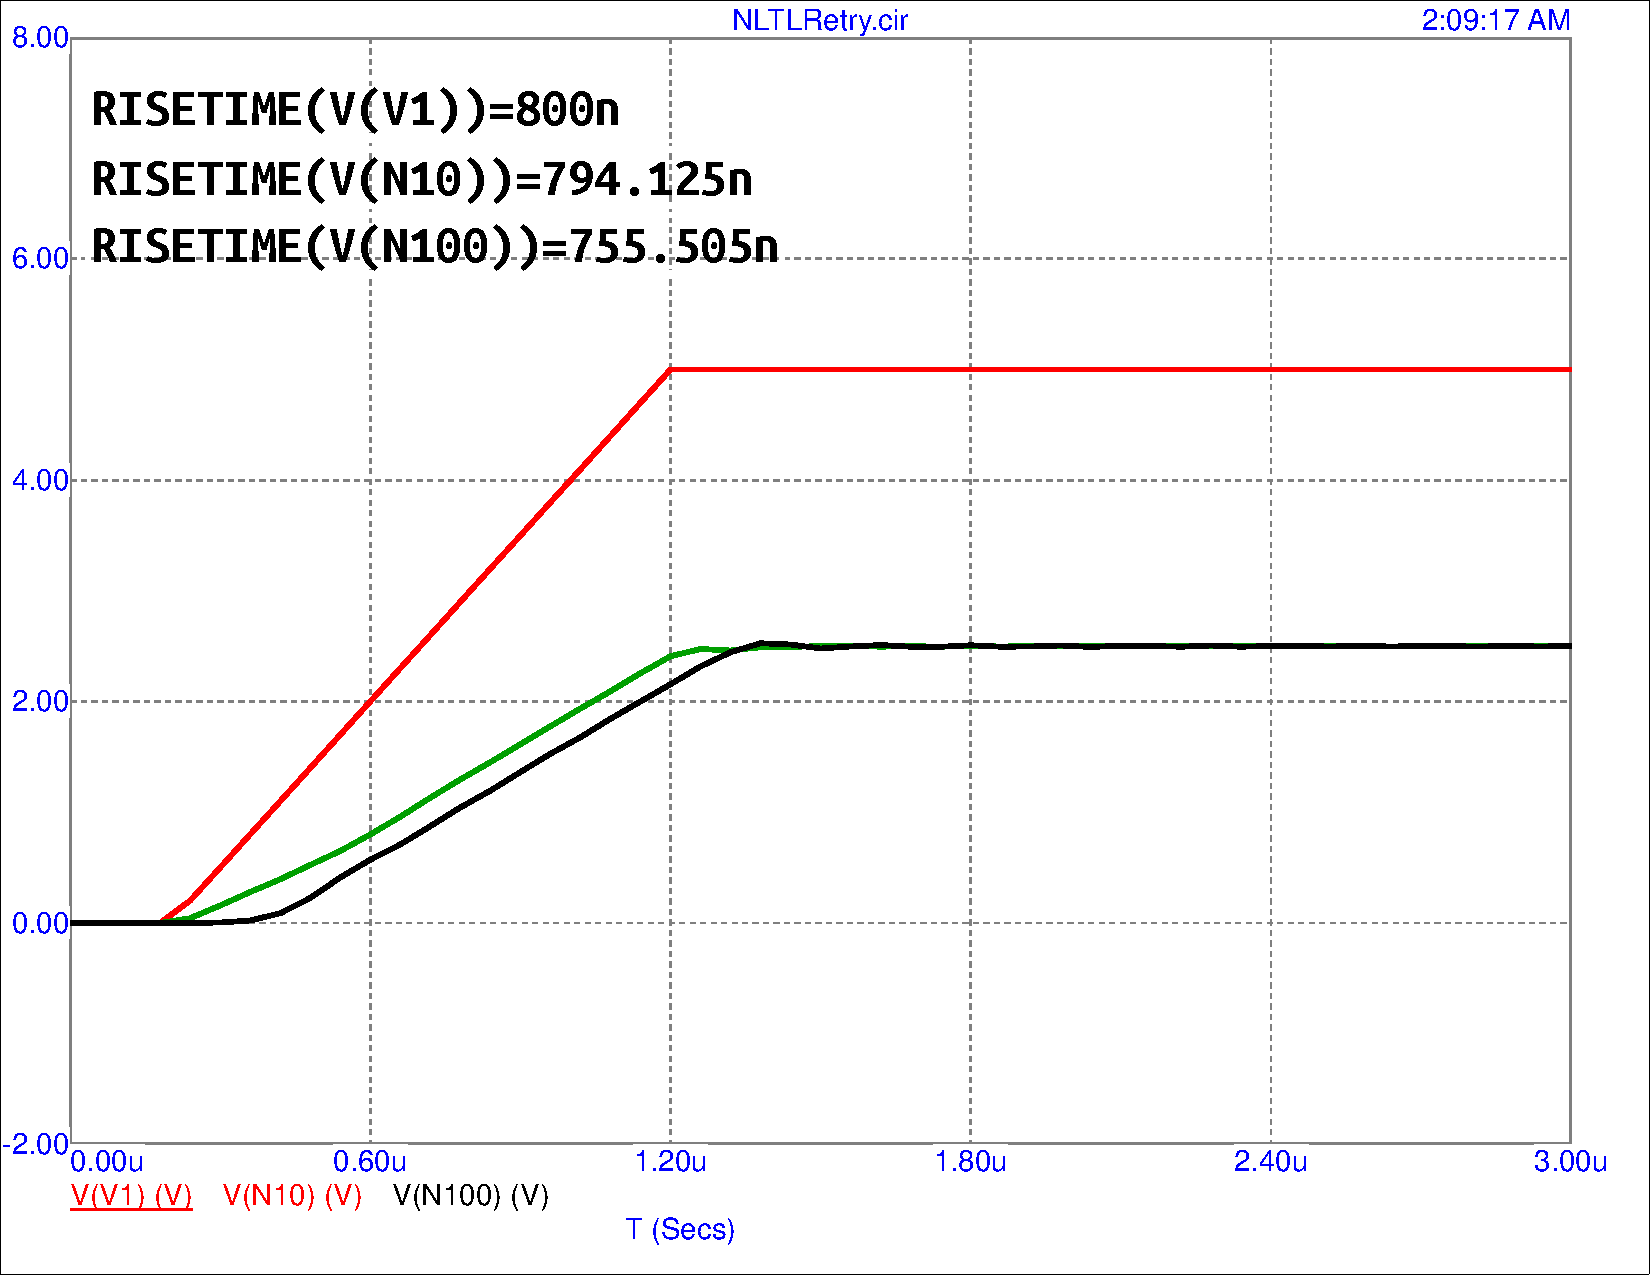
\includegraphics[width=0.45\textwidth,page = 1]{risetimeGuessNOLoss.pdf}
\caption{\ Rise time at source, node 10 and node 100 simulated with no resistive loss
}\label{fig:riseNoLoss}
\end{figure}

In figure \ref{fig:riseWithLoss}, we add the series DC resistance of the
inductor $(R_s \approx 122m\Omega)$ and the $1m\Omega$ resistance of the BBY40. 
From this, we see that not much has changed in this model and in fact we see an
increased sharpening effect if anything. We do notice however, that the
amplitude of the wave is much more attenuated at our $100^{th}$ node. This would
lead us to expect a decrease in the pulse sharpening in the circuit instead of a
relatively constant value due to the lessened effect on varactor capacitance as
the pulse climbs.

\begin{figure}[htb]
\centering
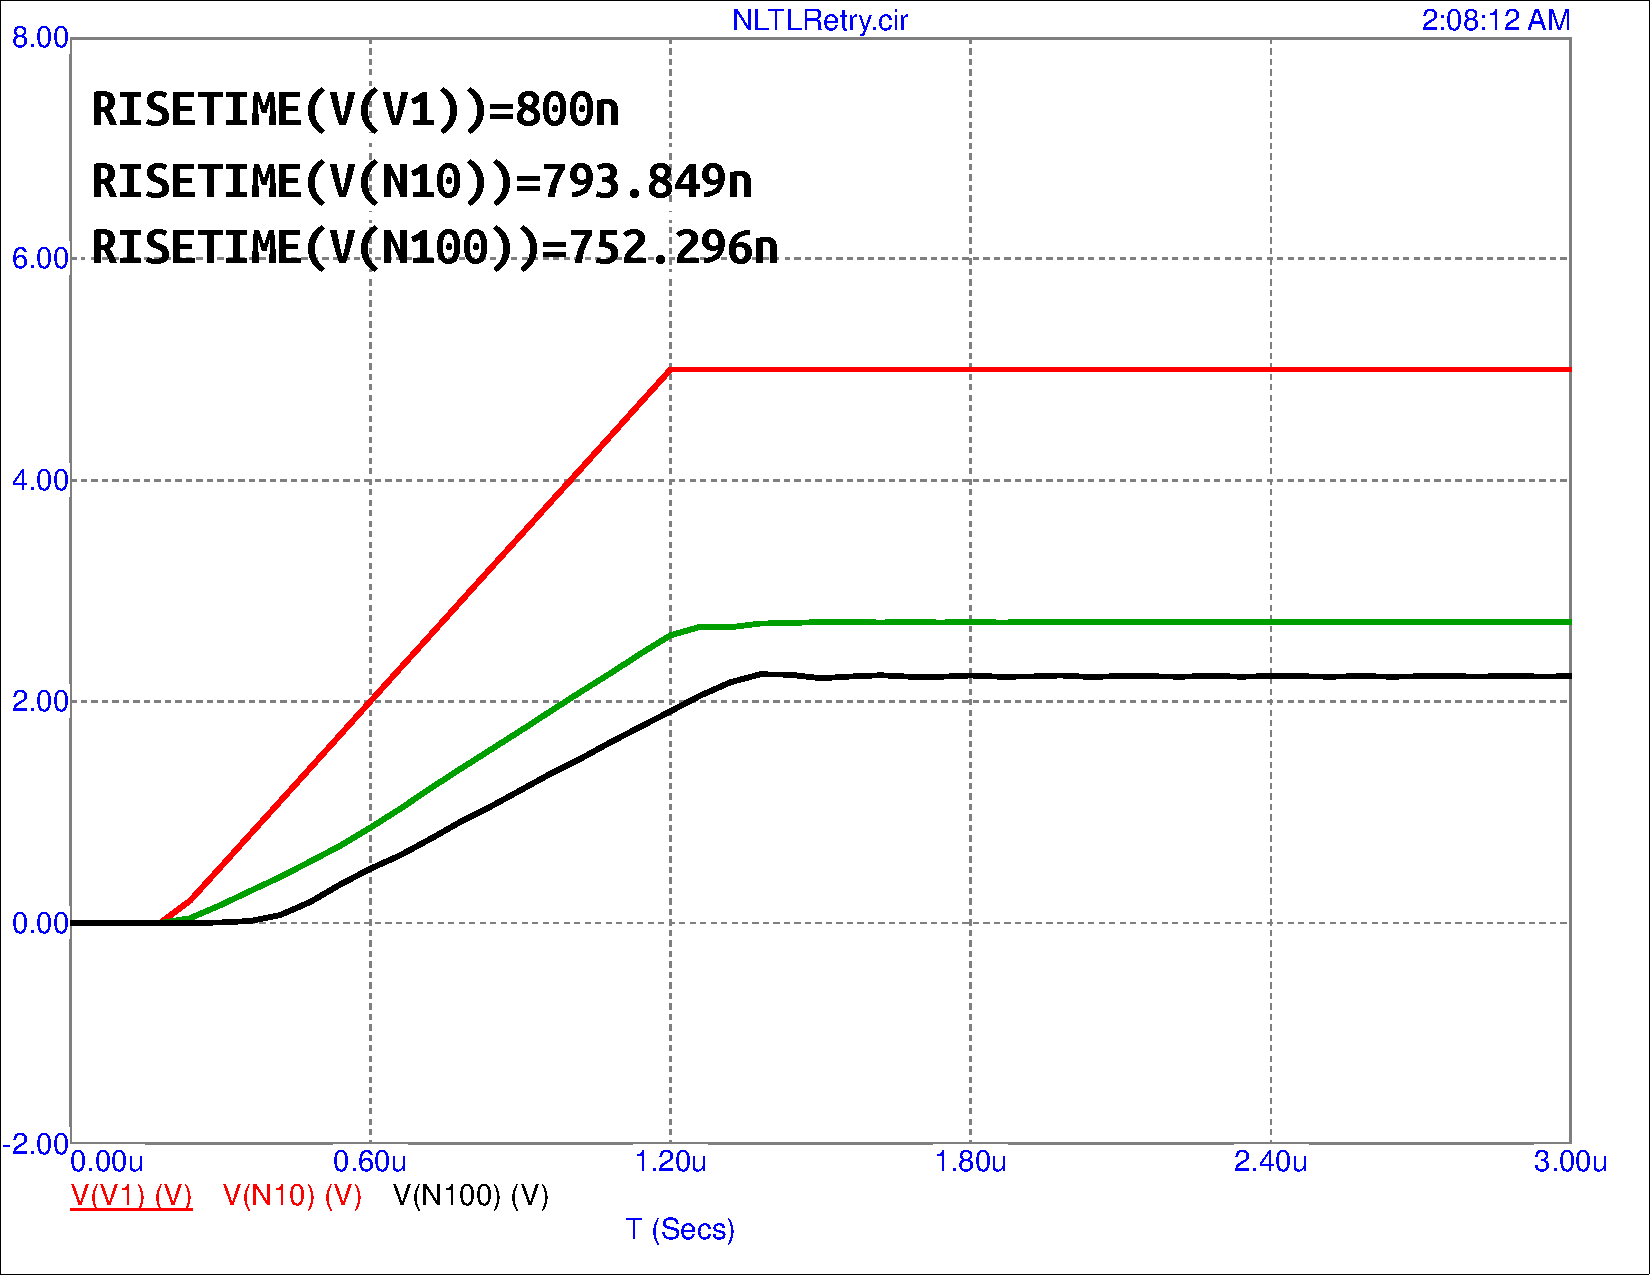
\includegraphics[width=0.45\textwidth,page = 1]{risetimeGuessWLoss.pdf}
\caption{\ Rise time at source, node 10 and node 100 simulated with resistive loss of $0.122\Omega$ per ladder section 
}\label{fig:riseWithLoss}
\end{figure}

 
 Figure \ref{fig:RiseVsLineVsBias} explores the effect of different biasing on
 our line as well as how long a line we can practically use for sharpening
 purposes. As our DC resistance grows with our line length, we expect our
 amplitude to keep dropping. As the amplitude of the traveling wave is reduced,
 we effectively trace out less of our varactor CV curves. Due to this, the CV
 relationship will begin to look more and more linear as we add ladder sections
 to our design. We have used a parametric plot to show the limits of this pulse
 sharpening as we increase  the line length and plotted rise-time vs. DC bias
 for each $10^{th}$ node of the ladder. The input pulse used in this case was
 $400ns$.

\begin{figure}[htb]
\centering
\includegraphics[width=0.4\textwidth,page = {3}]{RiseTimeVsDCBIASVsLength.pdf}
\caption{\ Risetime Vs. Line Length vs. DC Bias Voltage 
}\label{fig:RiseVsLineVsBias}
\end{figure}






\section{Board Design} 


In order to test all these simulated values we designed a discrete version of
our transmission line using Altium Designer. We emphasized traces being as short
as possible and used Altium's built-in impedance profile tool to match our path
between each pair of SMA connectors to $50\Omega$. The circuit we constructed is
shown assembled in figure \ref{fig:assembled}.


\begin{figure}[htb]
\centering
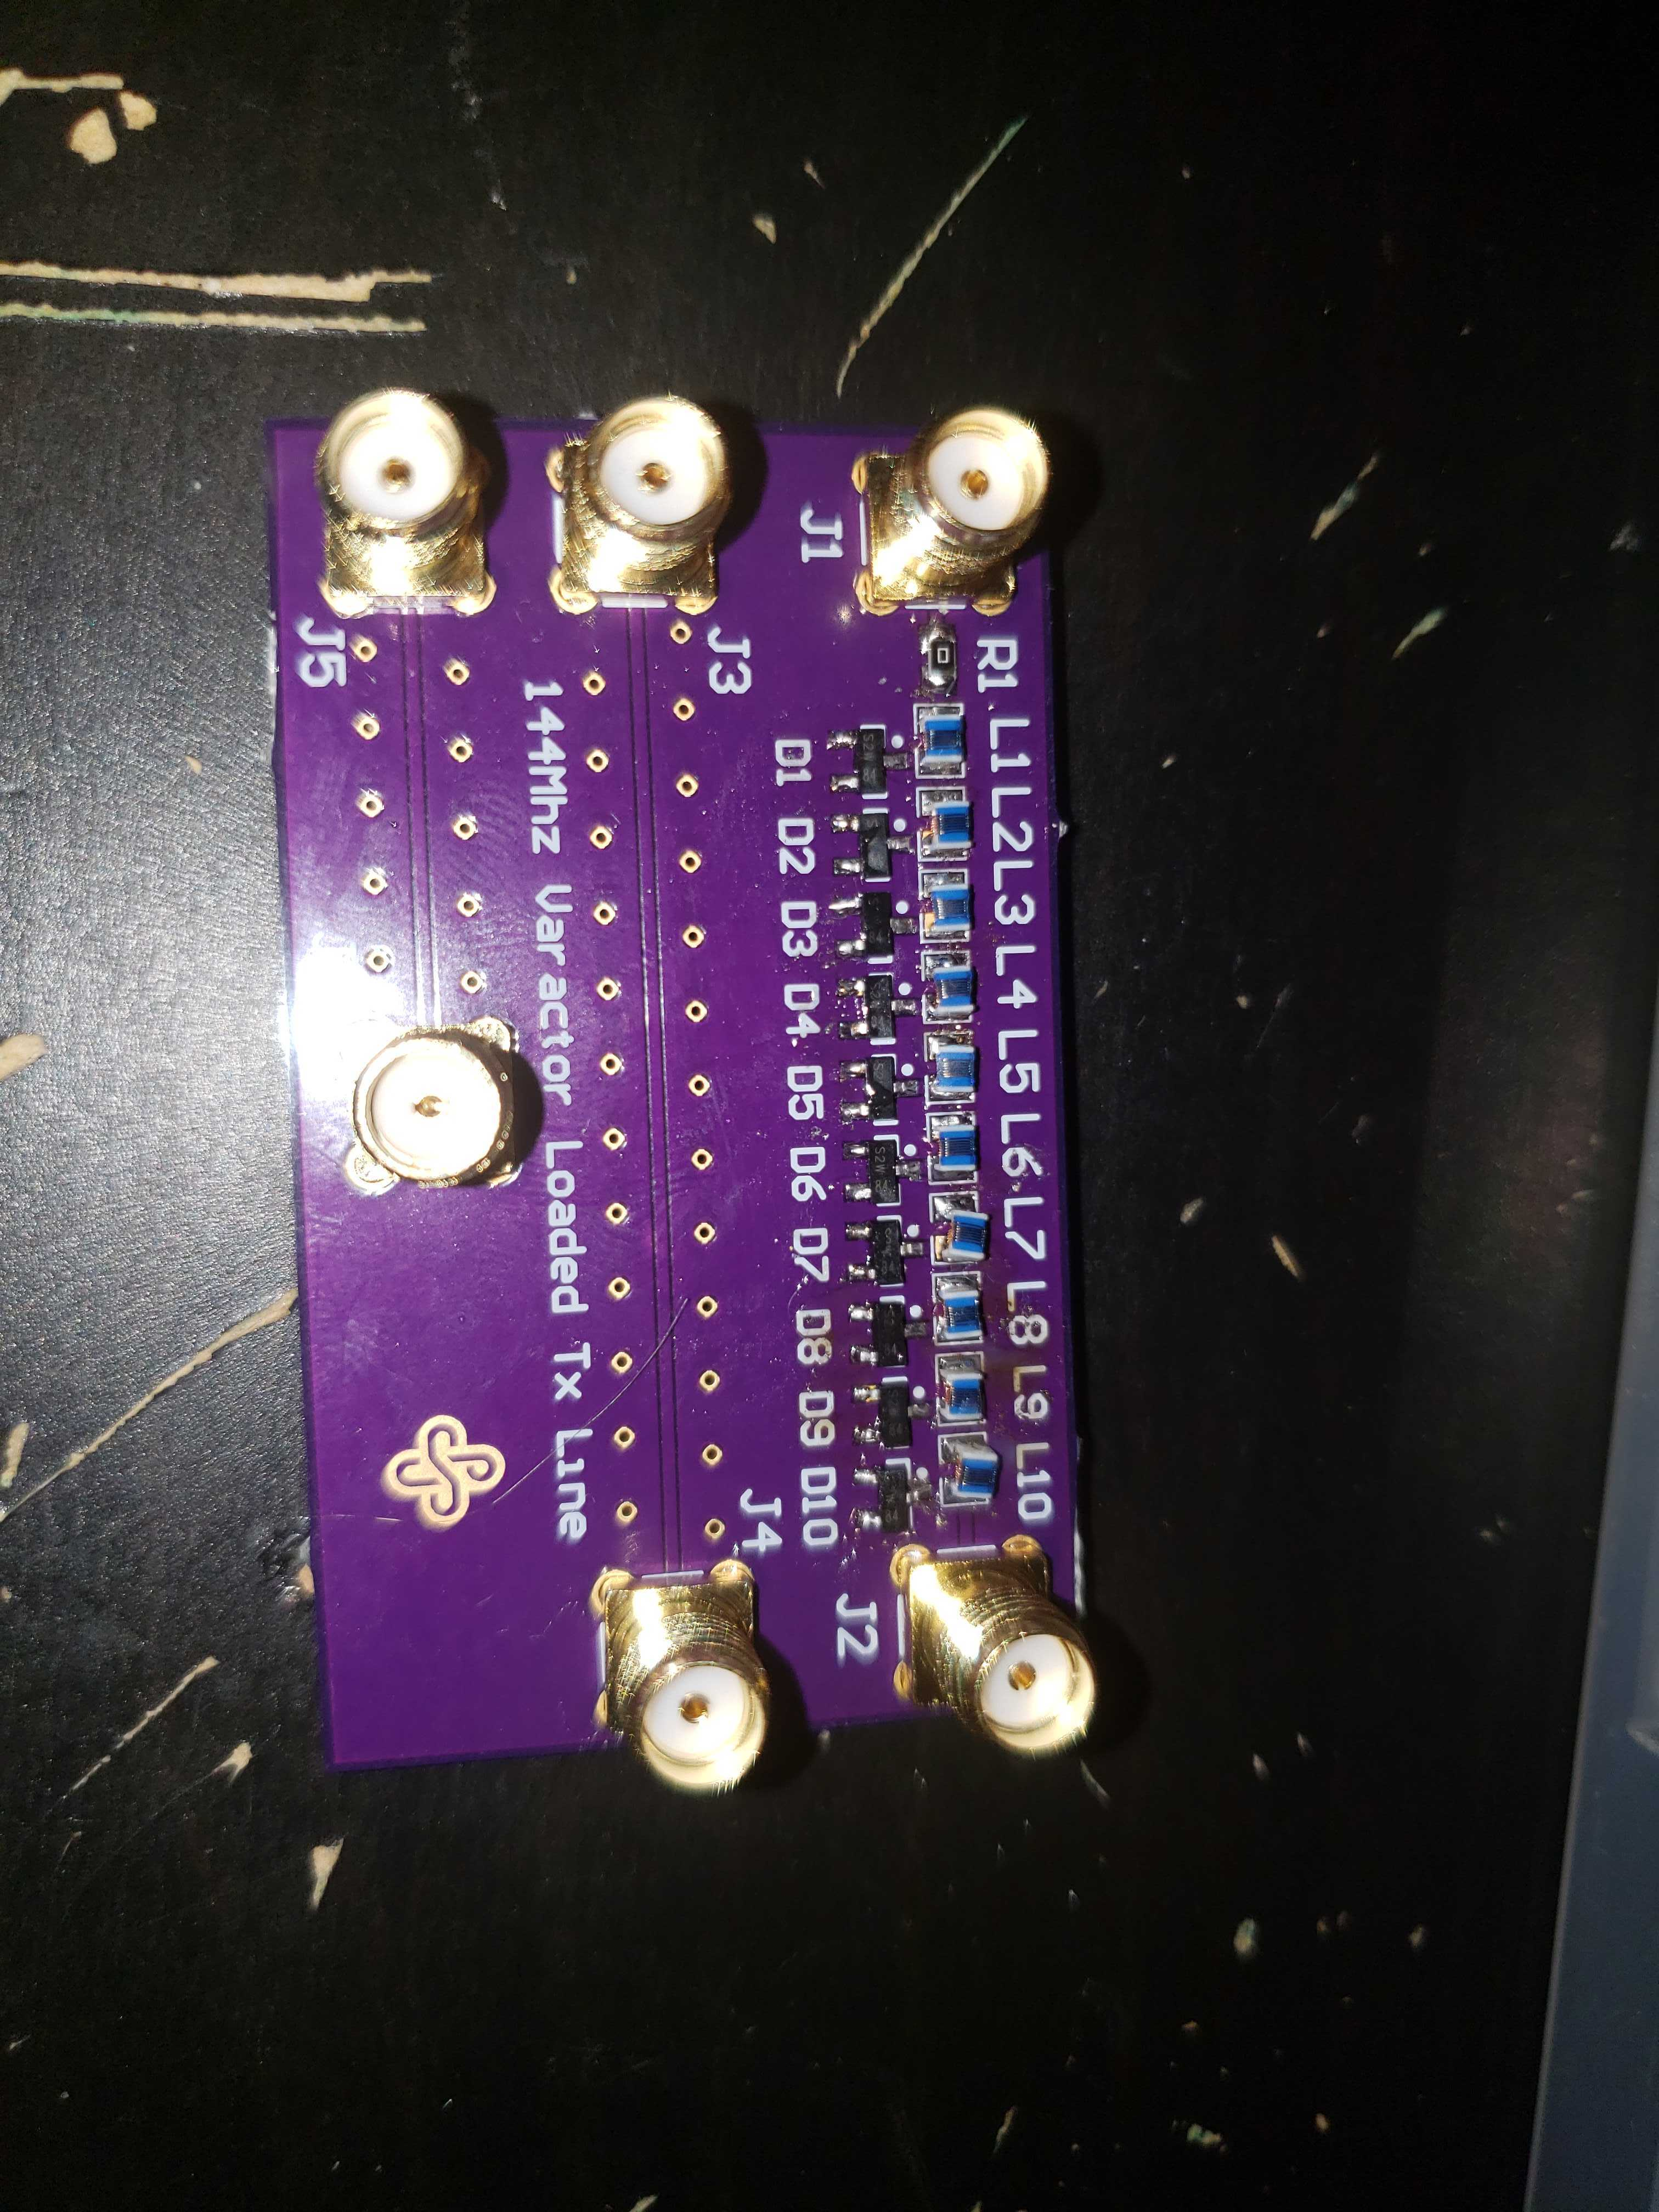
\includegraphics[width=0.3\textwidth, angle = 90]{AssembledBoard.jpg}
\caption{\ Assembled Tx Line Board made for 144Mhz
}\label{fig:assembled}
\end{figure}





\section{ Measurement Results }






\subsection{Varactor CV Curves}\label{subsec:CVCurves}

To measure and find the capacitance vs Voltage of our chosen varactors we
created a small ugly style circuit based on a design by W2AEW. Two 100k
resistors are added to limit current flowing to the power supply. A ceramic
capacitor of value much greater than our varactor is placed to protect the meter
from excessive voltage. Since this larger capacitance is in effectively in
parallel with our varactor, our meter measurement is approximately only the
capacitance of the varactor diode itself.

\begin{figure}[htb]
\centering
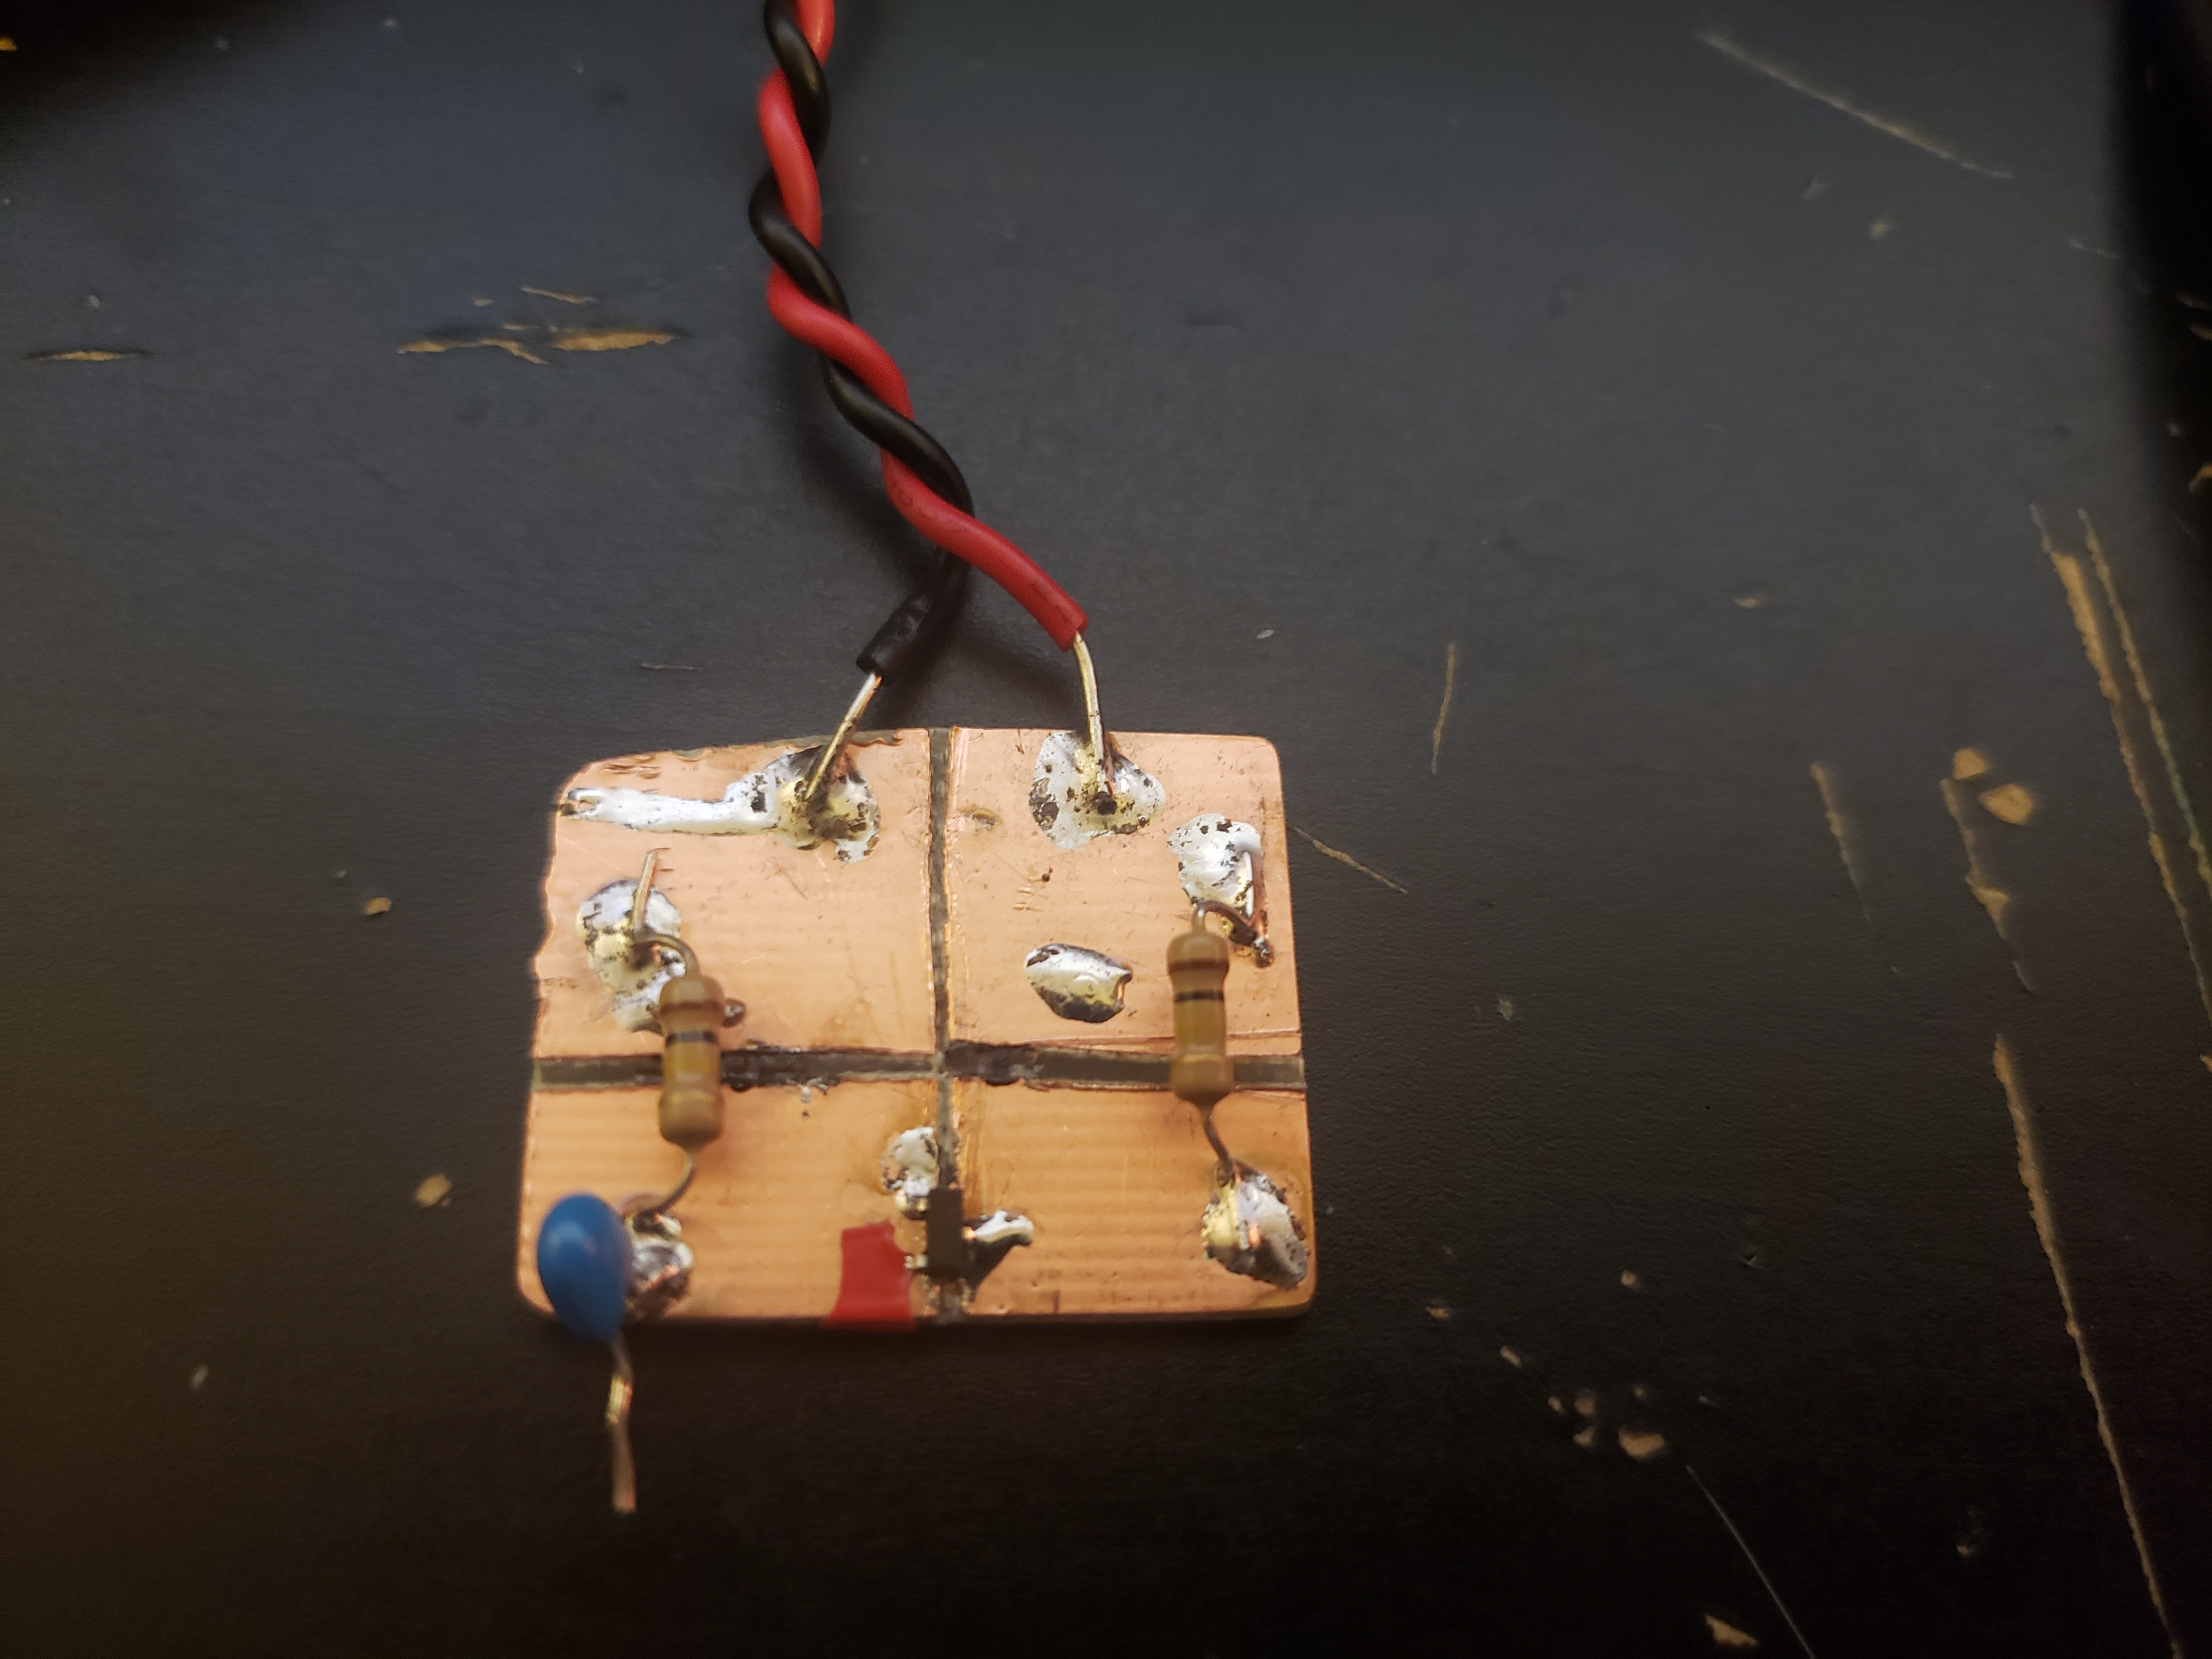
\includegraphics[width=0.45\textwidth]{BBY40_capacitance_testfixture}
\caption{\ Test Fixture used for plotting CV Curve of BBY40
}\label{fig:CVTestFixt}
\end{figure}



Through use of this fixture, we were able to generate the curves shown in
figures \ref{fig:BBY40CV} and \ref{fig:SMV1249CV}. These were in close agreement
to curves found on datasheets for the BBY40 and SMV1249 respectively.
 
\begin{figure}[htb]
\centering
\includegraphics[width=0.45\textwidth]{bbY40CV}
\caption{\ Measured CV Characteristics of BBY40 
}\label{fig:BBY40CV}
\end{figure}
 
 
\begin{figure}[htb]
\centering
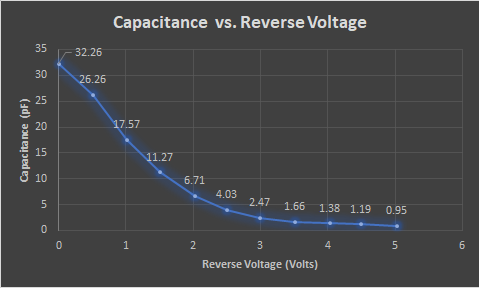
\includegraphics[width=0.45\textwidth]{SMV1249_CV}
\caption{\ Measured CV Characteristics of SMV1249 
}\label{fig:SMV1249CV}
\end{figure}


\subsection{AC Response}\label{ACMeasResults}


\begin{figure}[htb]
\centering
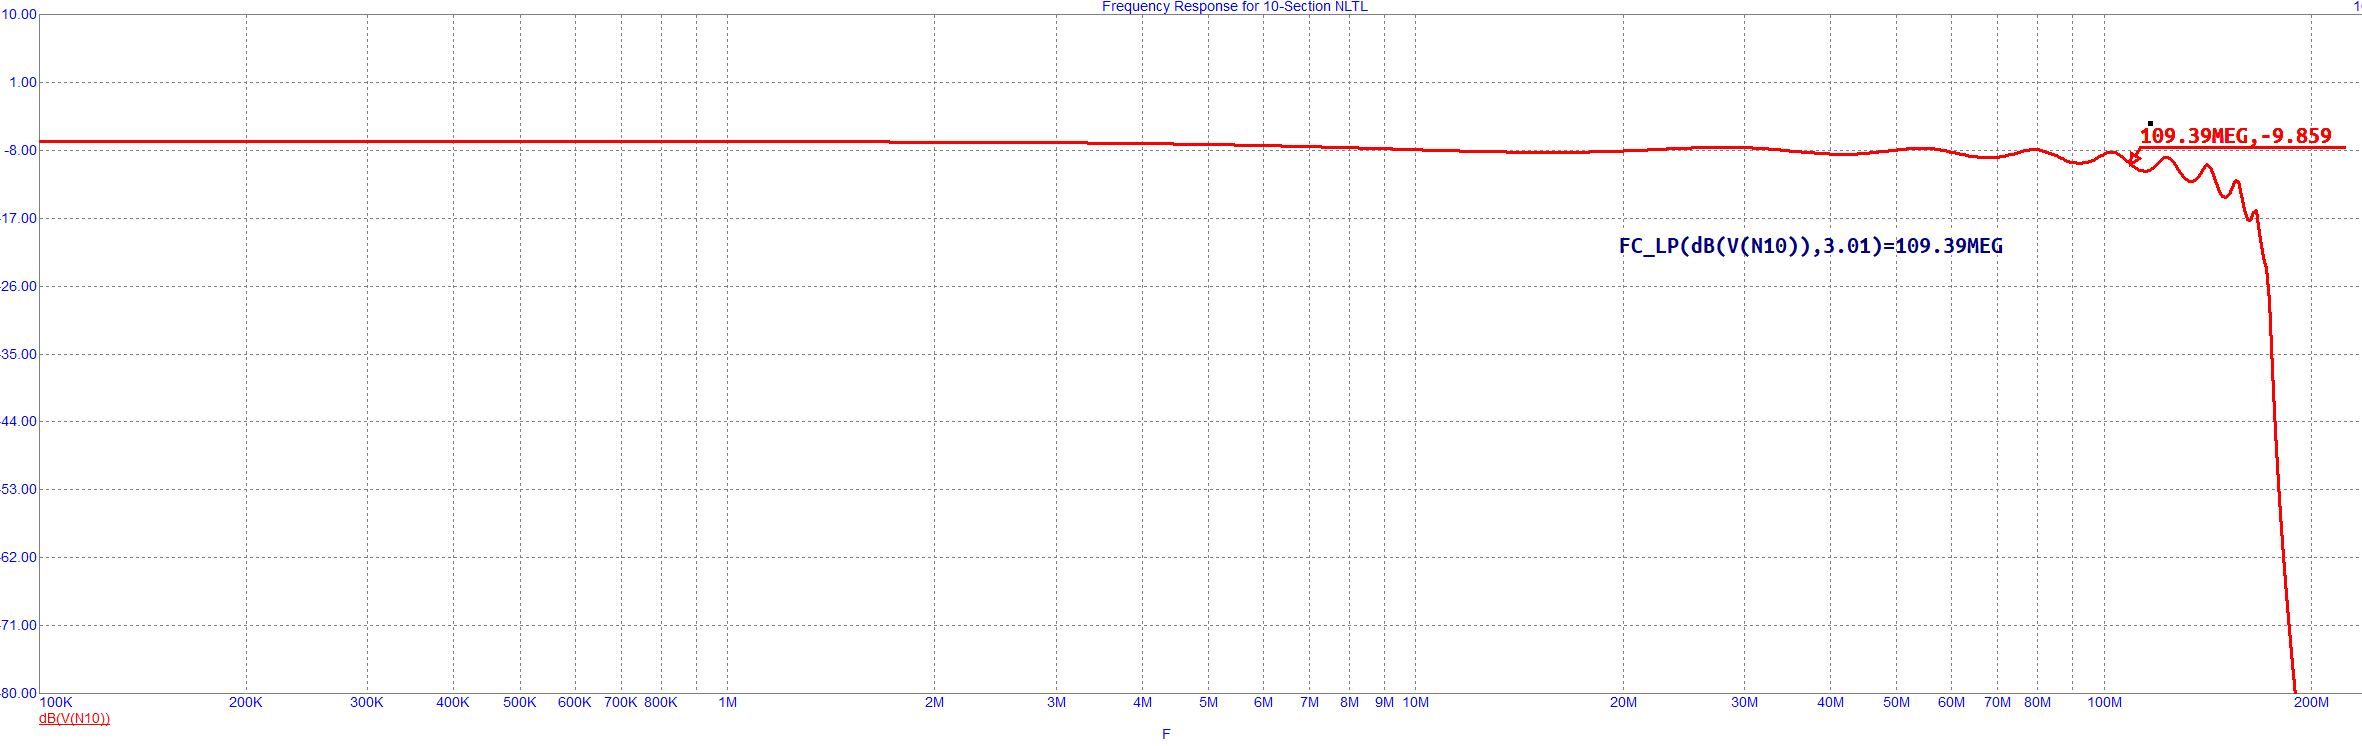
\includegraphics[width=0.35\textwidth,angle = -90]{ACResponseB1}
\caption{Simulated AC Response for Board 1}
\label{fig:simACBoard1}
\end{figure}

\begin{figure}[htb]
\centering
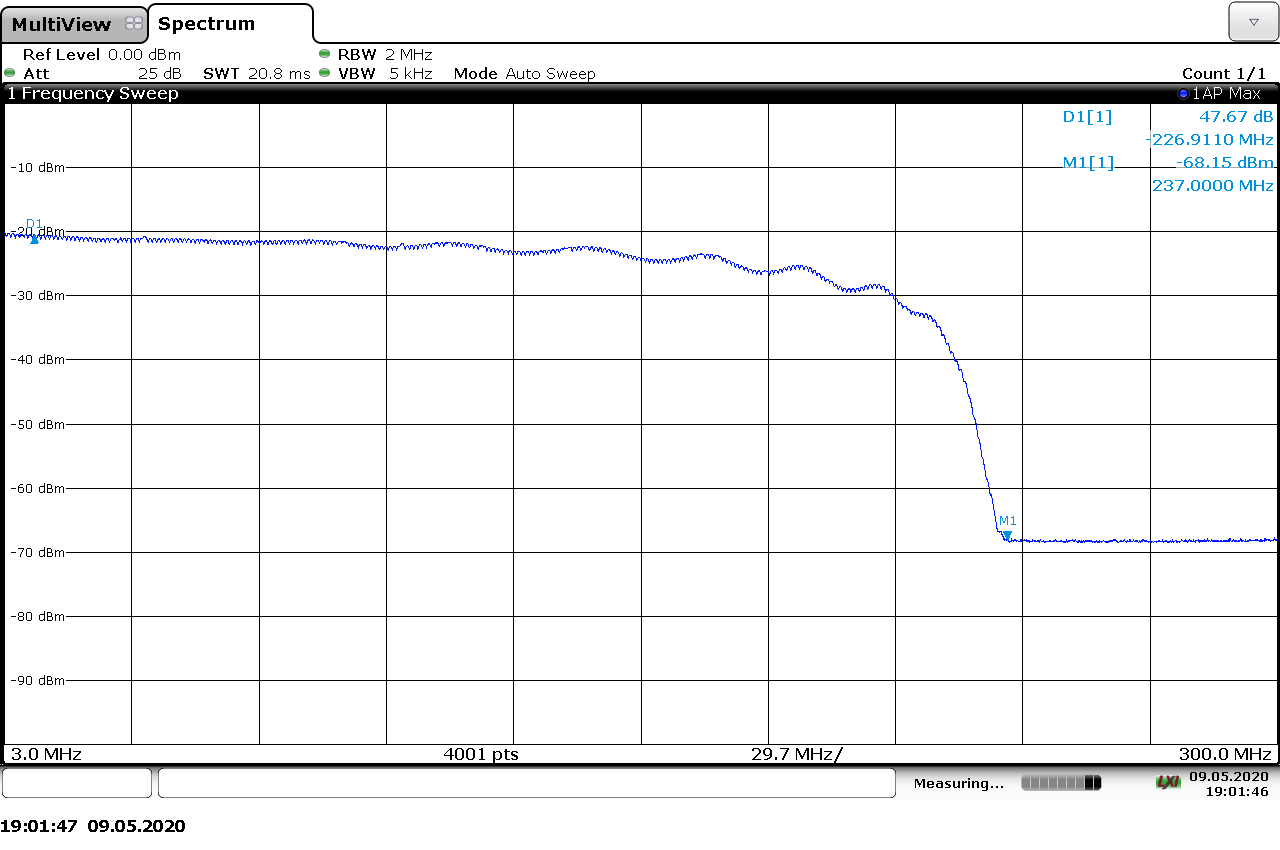
\includegraphics[width=0.45\textwidth]{MeasuredACResponseB1.png}
\caption{Measured Frequency Response for Board 1 (L= 56nH)}
\label{fig:MeasACBoard1}
\end{figure}





\subsection{Rise Time}\label{RiseTimeMeasResults}

We had great difficulty in measuring rise time of our circuit and the main
problems we faced were not understanding the theory well enough have do proper
testing. While our components were chosen on the basis of working at 144Mhz, we
failed to see that driving our circuit below this bandwidth and performing
similar simulations may be adequate to prove rise time performance increase.
Another complication was keeping in mind the biasing conditions of the
varactors. We did not design for a port in which to introduce a dc bias to our
circuit and relied on equipment being able to accomplish this. Care must be
taken when using analog generators to supply the DC bias to the circuit. Our
particular model begins sweeping with a negative bias before reaching a positive
one. This effectively puts the varactors into forward bias and allows them to
hold a charge.






\begin{figure}[htb]
\centering
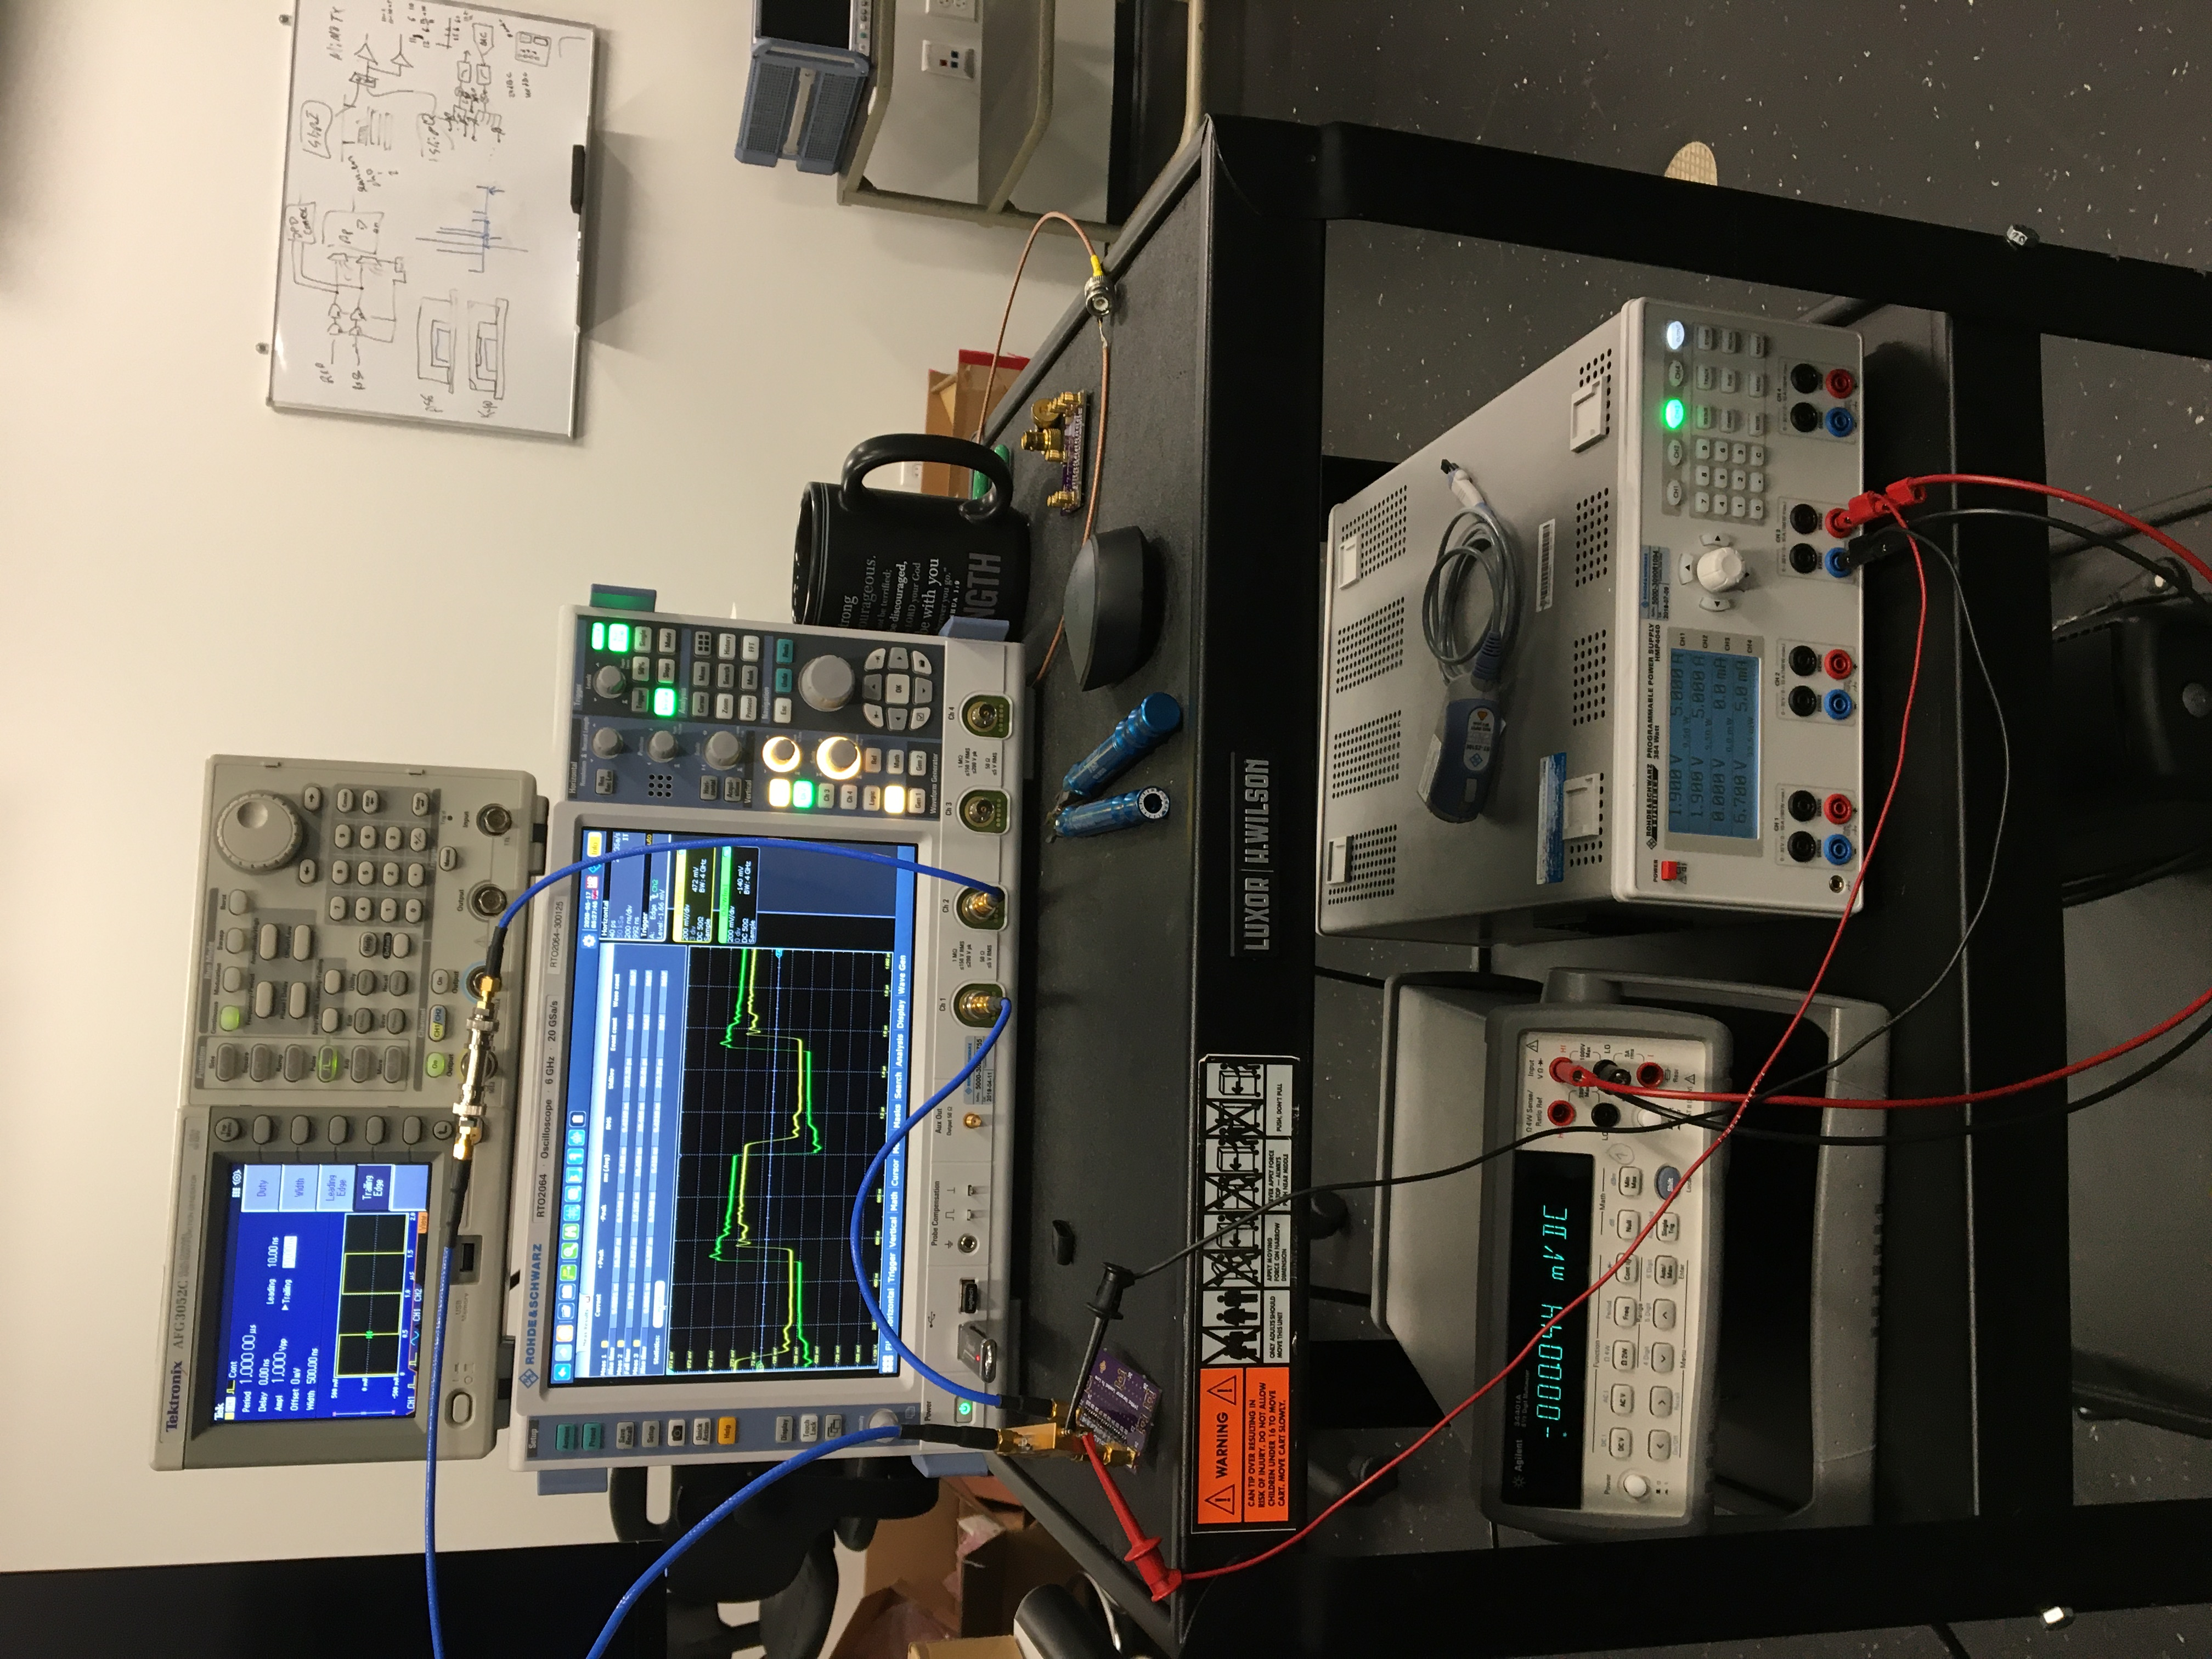
\includegraphics[width=0.45\textwidth,angle = -90]{SetupWithBiasing.JPG}
\caption{Test Setup for Measuring Risetime With Bias}
\label{fig:SetupWBiasing}
\end{figure}


\begin{figure}[htb]
\centering
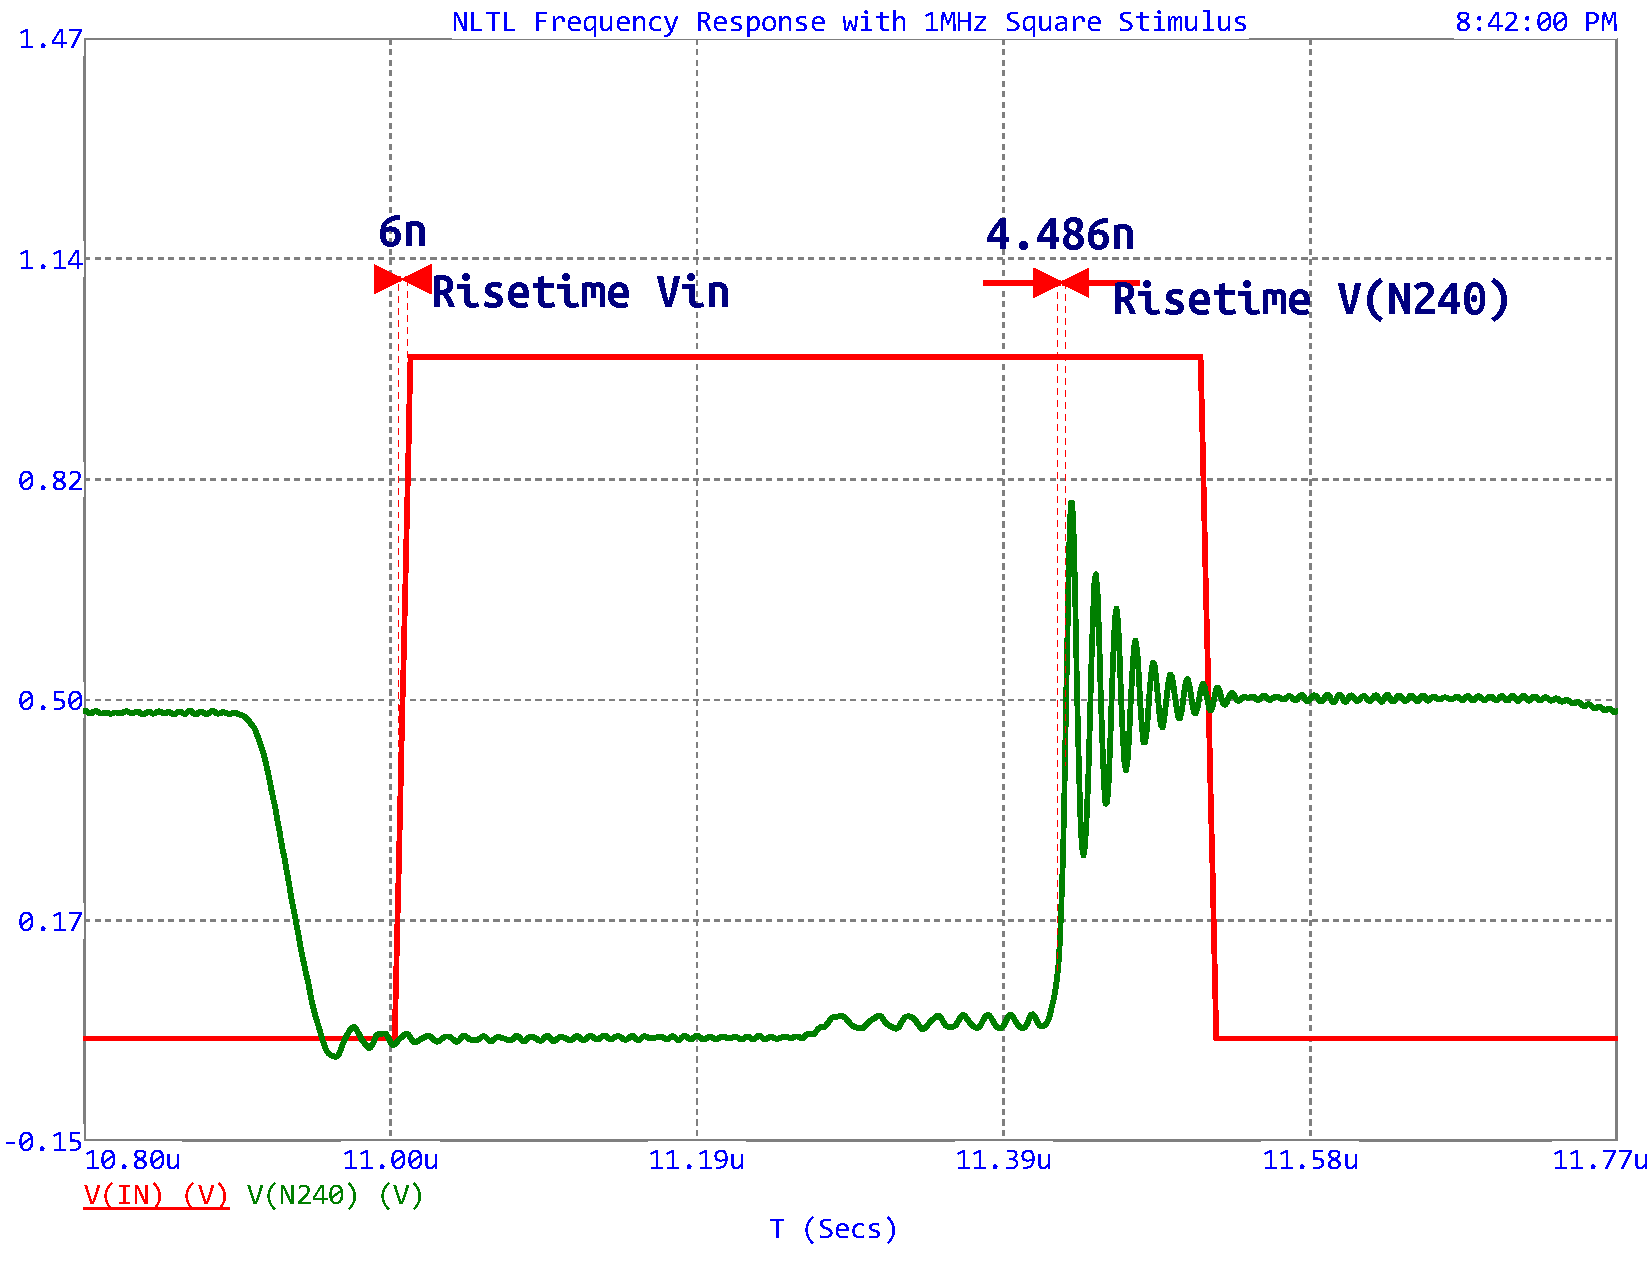
\includegraphics[width=0.45\textwidth]{Probed_Input_N10_N240_NoSeriesResistance}
\caption{Simulated Risetimes for Input pulse, $10^{th}$ node, and the $240^{th}$ node}
\label{fig:probedNoResistance}
\end{figure}


\begin{figure}[htb]
\centering
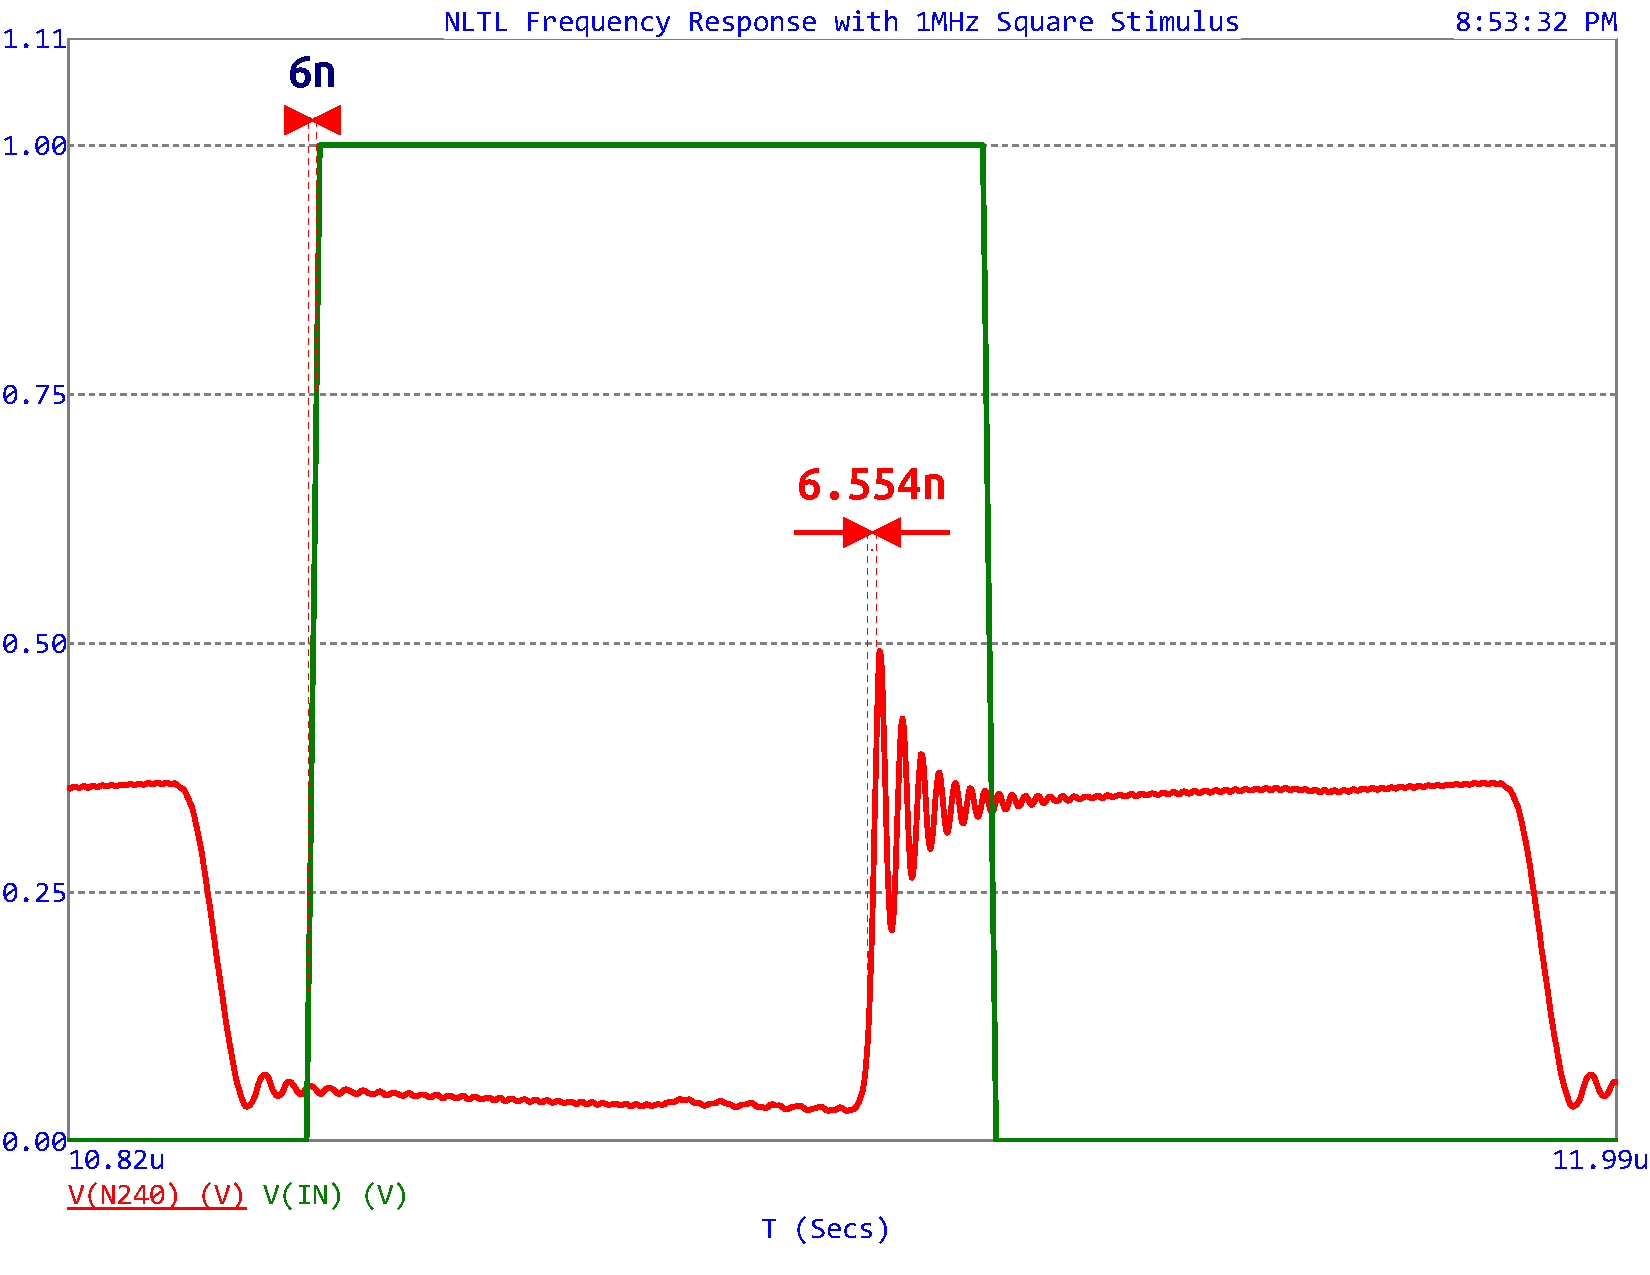
\includegraphics[width=0.45\textwidth]{Probed_Input_N10_N240_With_SeriesResistance}
\caption{Accounting for Series Resistance shows that there is a certain point where no more sharpening takes place}
\label{fig:probedWithResistance}
\end{figure}


\begin{figure}[htb]
\centering
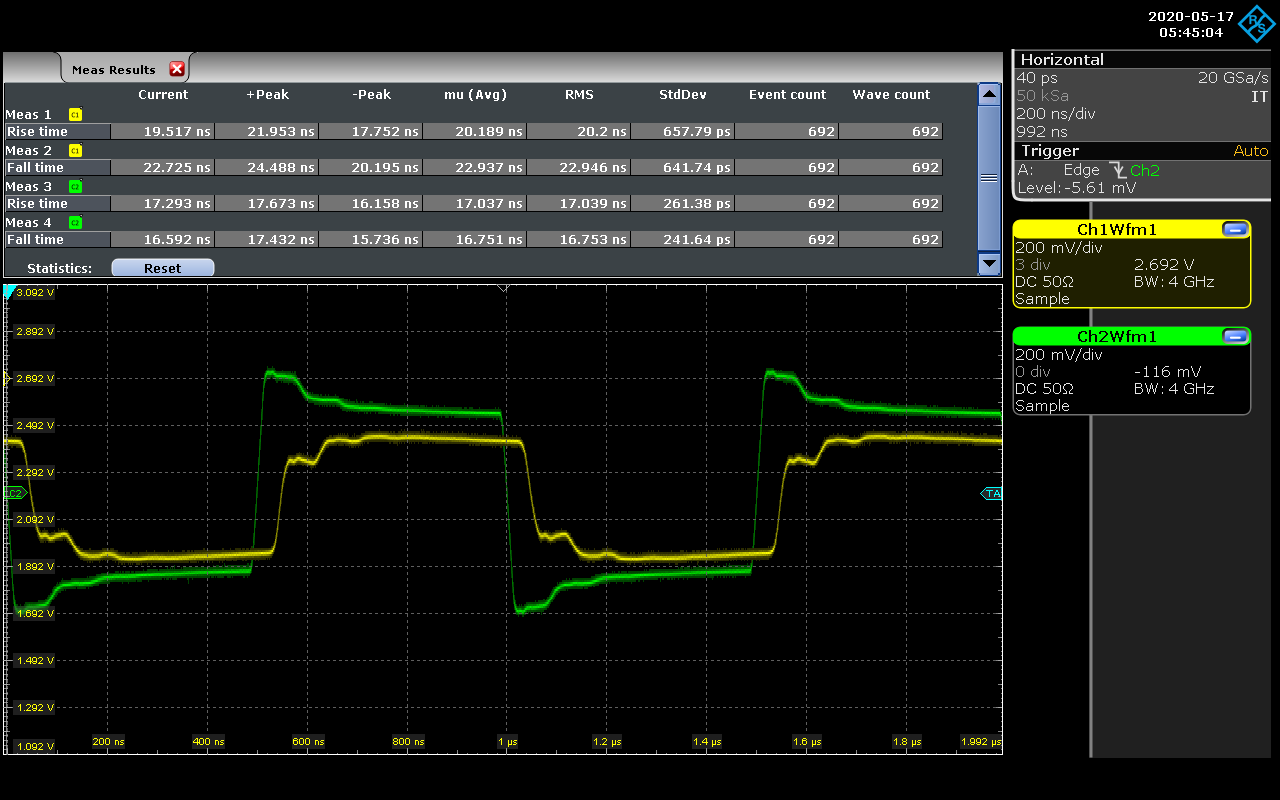
\includegraphics[width=0.45\textwidth]{MeasuredSquareResponseB1.png}
\caption{Risetime Measurement from Board 1 (L=56nH)}
\label{fig:MeasuredSquareGeneric}
\end{figure}

\begin{figure}[htb]
\centering
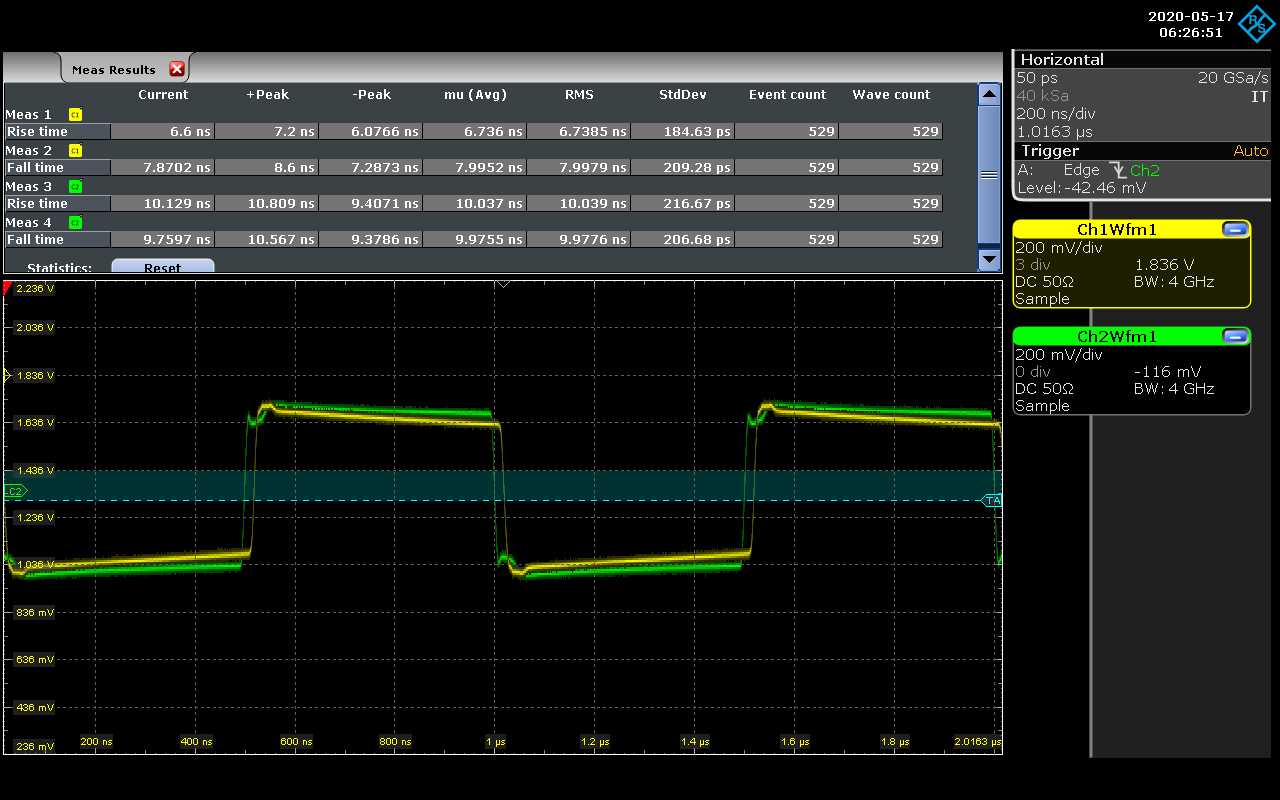
\includegraphics[width=0.45\textwidth]{MeasuredSquare1VBiasB1.png}
\caption{Measured Risetime with 1V DC Bias}
\label{fig:MeasuredSquare1VBiasB1}
\end{figure}

\begin{figure}[htb]
\centering
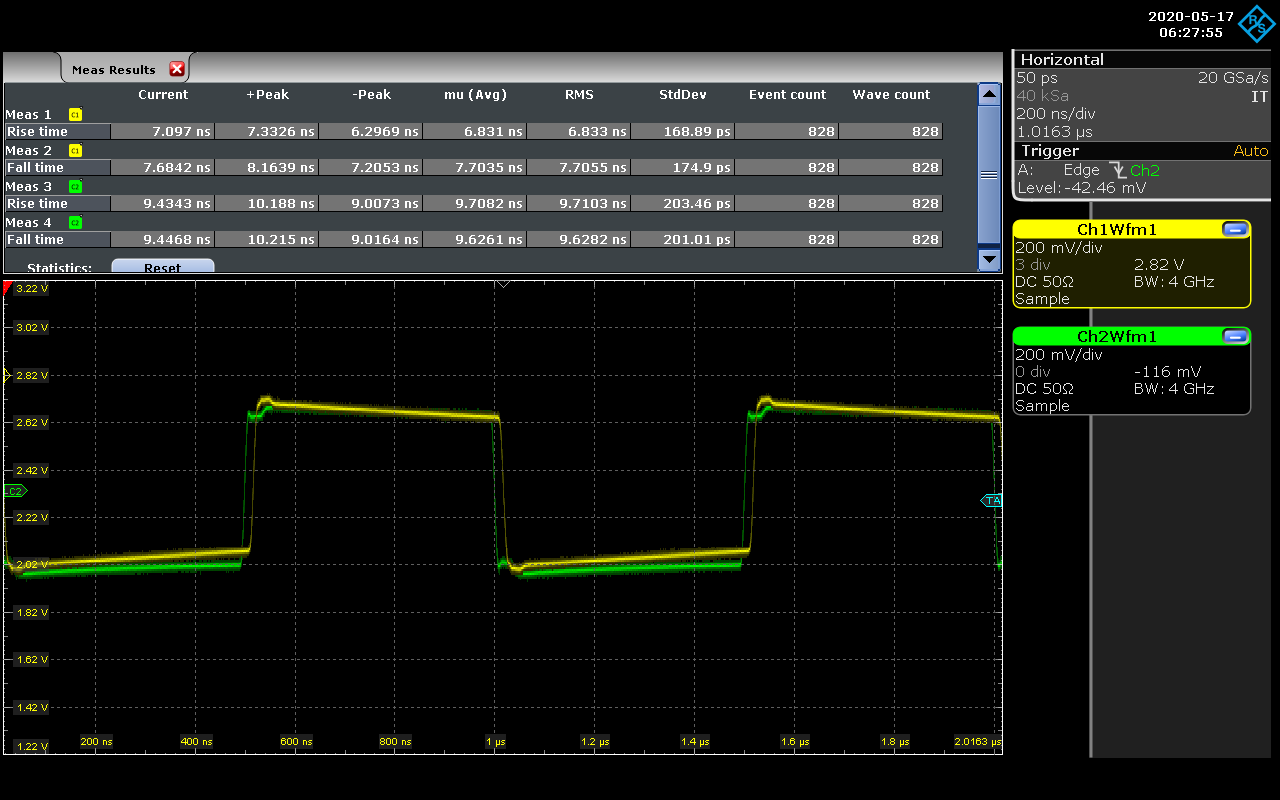
\includegraphics[width=0.45\textwidth]{MeasuredSquare2VBiasB1.png}
\caption{Measured Risetime with 2V DC Bias}
\label{fig:MeasSquare2VBiasB1}
\end{figure}


\begin{figure}[htb]
\centering
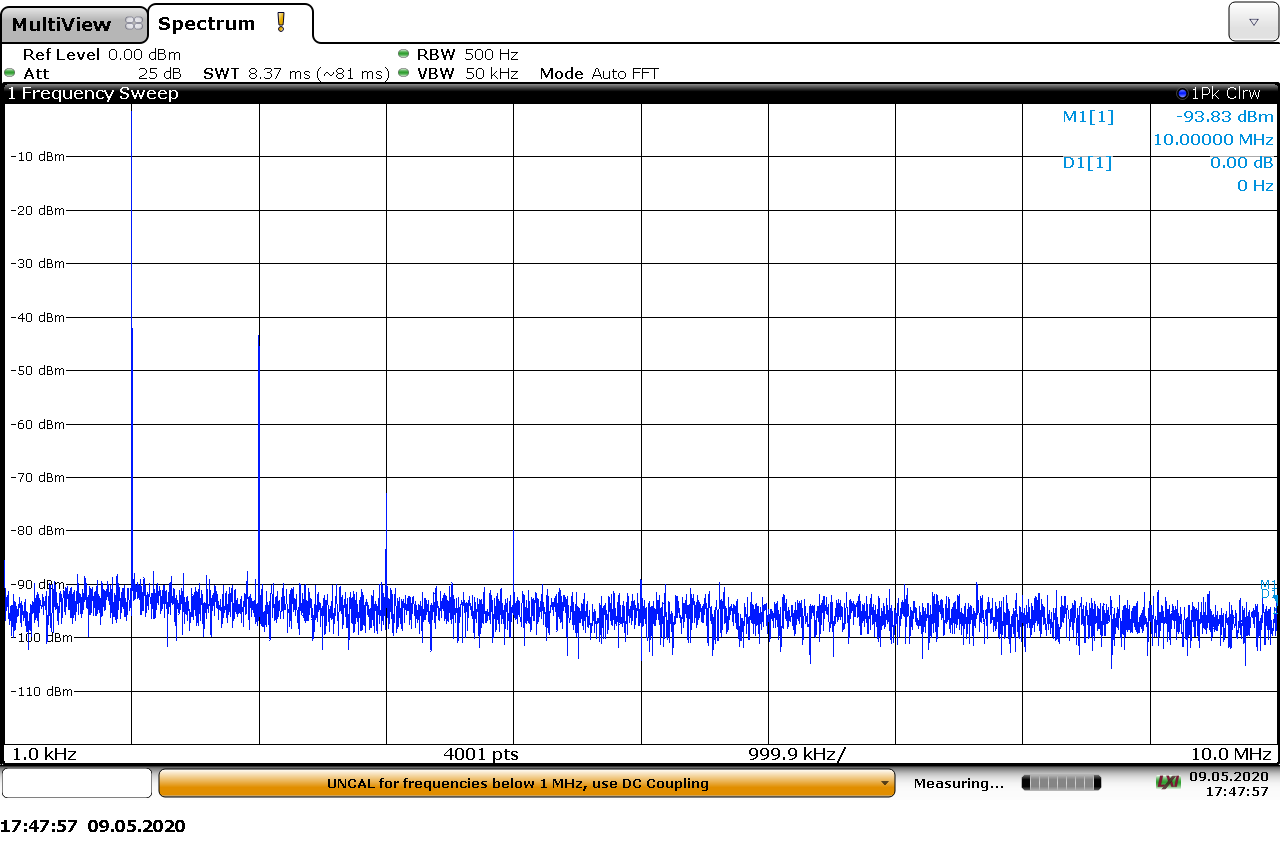
\includegraphics[width=0.45\textwidth]{MeasuredSpectrum.png}
\caption{}
\label{fig:MeasSpec}
\end{figure}

\begin{figure}[htb]
\centering
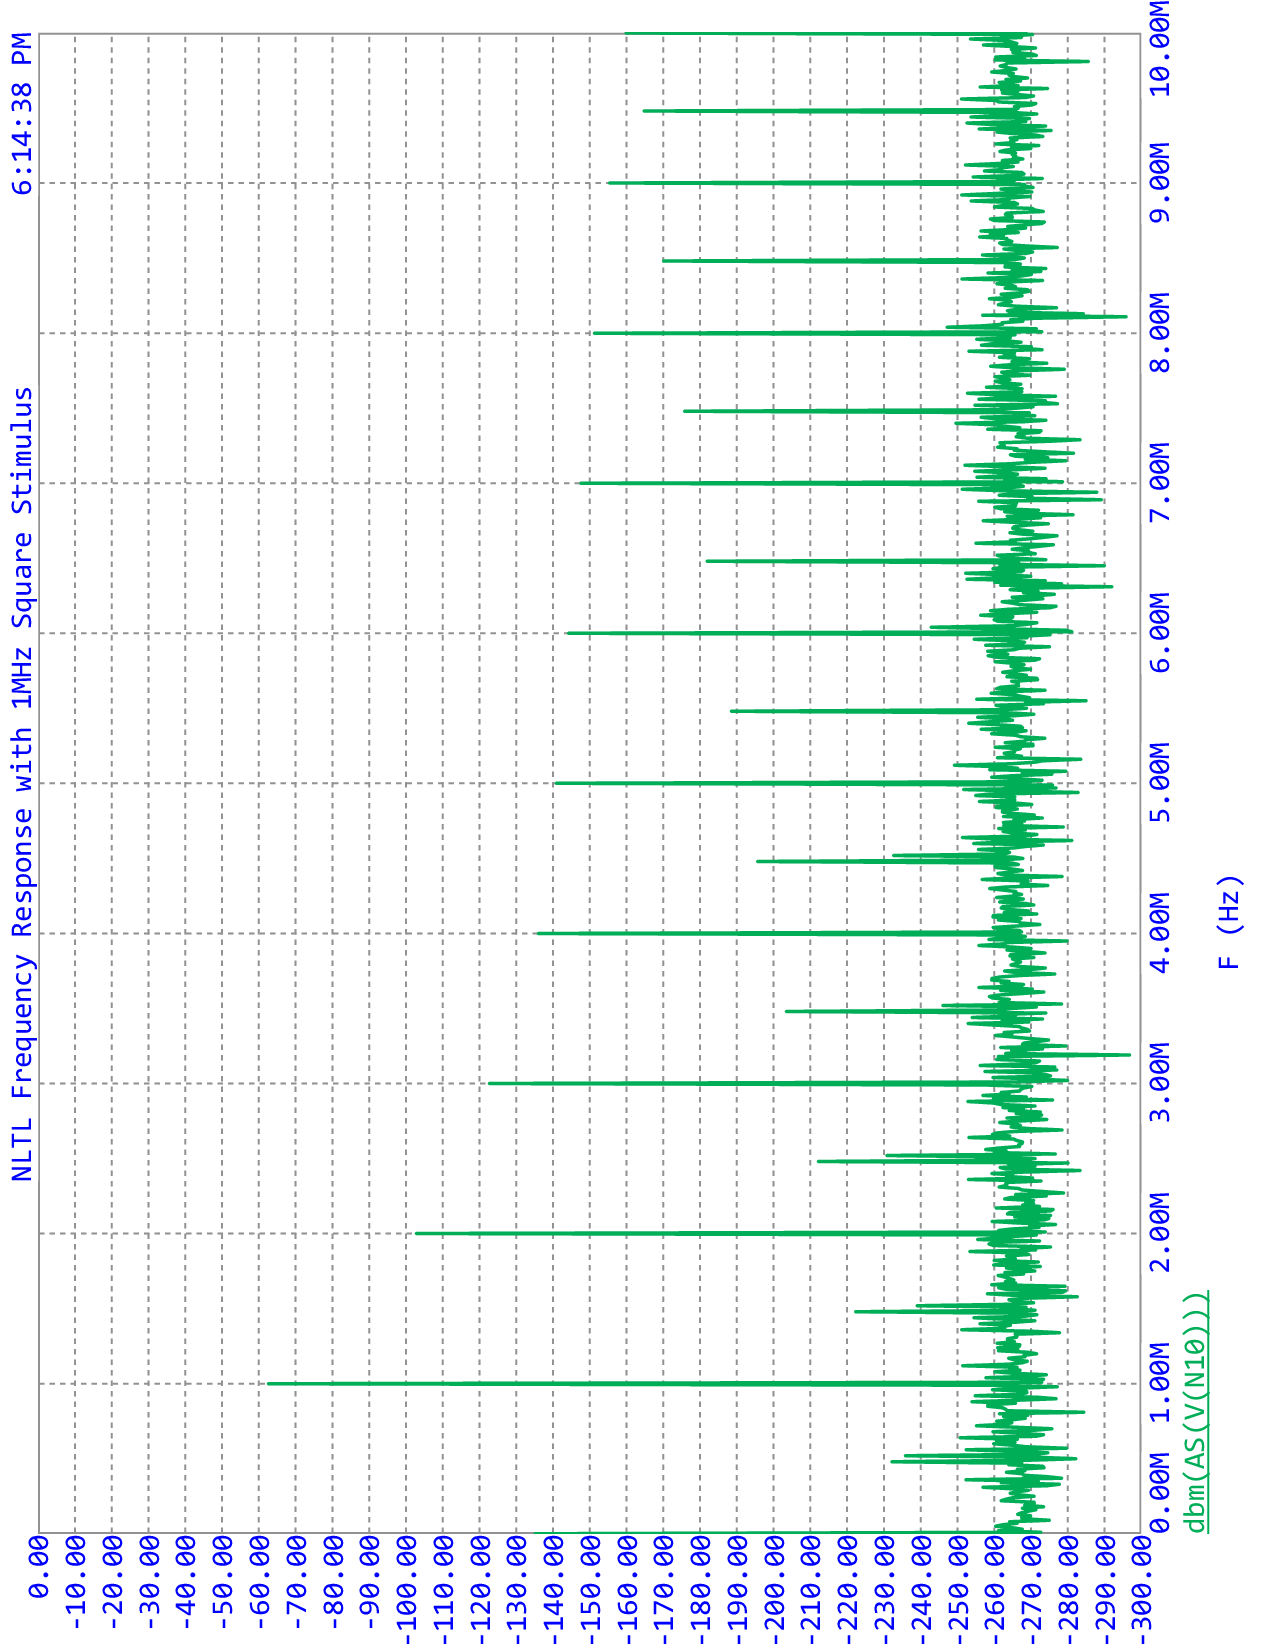
\includegraphics[width=0.38\textwidth,angle=-90]{SimulatedSpectrum.png}
\caption{Expected Power Spectrum when DUT fed with 1Mhz 1Vpp Sine Wave}
\label{fig:SimSpec}
\end{figure}




\subsection{S-parameters}


In figure \ref{fig:sparamSchem} shows the schematic used to measure and compare
our measured s-parameters taken through a NanoVNA to our simulated circuit with
parasitics included. The NanoVNA data is imported through use of the n-port
components and define statements are utilized to calculate other parameters such
as generated power in dbm, VSWR, etc...


\begin{figure}[htb]
\centering
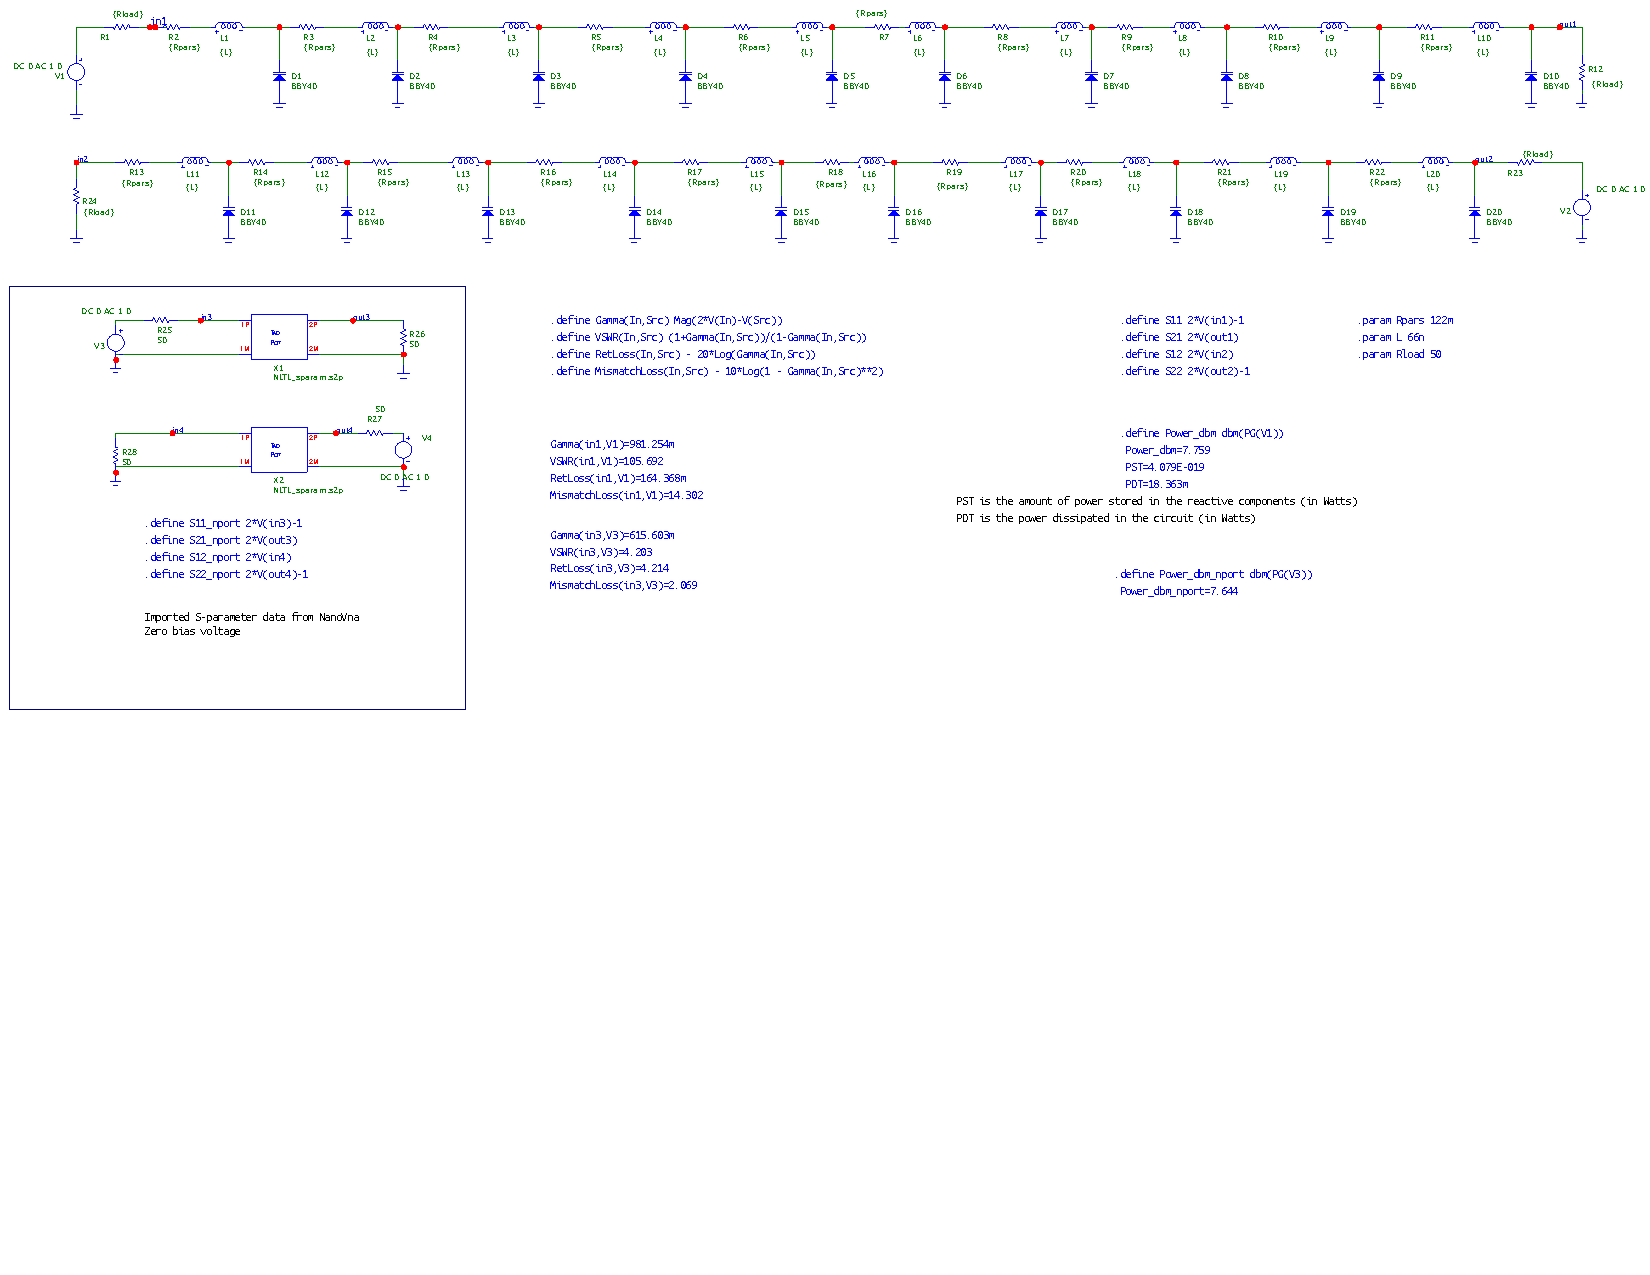
\includegraphics[width=0.45\textwidth,page = 1]{images/MostRecentSparamMeasSchem.pdf}
\caption{Schematic used to generate S-parameter plots. The top line measures S11 and S12, and bottom line measures S21 and S22. 
}\label{fig:sparamSchem}
\end{figure}


To produce figure \ref{fig:S11_S21}, we parameterized the values of our
parasitic elements in circuit and within the BBY40 model itself. We changed
these values to match our measured data more closely to see the accuracy of our
model. While we were able to achieve relatively agreeing data we still see a
large discrepancy in our S11 data. At 10MHz, we see a our measured data is
roughly $-10dbm$ lower than our expected simulation. This could be due to
incorrect modeling of our load impedances and requires further study. Some have
mentioned that when using NLTL's, there is bound to always be some impedance
mismatch due to the changing impedance caused by varactor capacitance
\cite{wilson1991pulse}. This may be the case here, but the issue is worth
further simulation.

\begin{figure}[htb]
\centering
\includegraphics[width=0.45\textwidth,page = 2]{Fixed_ZeroBias_Sparam_Sims.pdf}
\caption{\ Simulated vs. Measured $S_{11}$ and $S_{21}$. Corrections to make on next draft include more sensible scaling of axes
}\label{fig:S11_S21}
\end{figure}



\begin{figure}[htb]
\centering
\includegraphics[width=0.45\textwidth,page = 3]{Fixed_ZeroBias_Sparam_Sims.pdf}
\caption{\ Simulated vs. Measured Return Loss and VSWR
}\label{fig:VSWRandReturnLoss}
\end{figure}

In figure \ref{fig:VSWRandReturnLoss}, we see that our measured and simulated
are almost identical except for a sharp rise in VSWR near the resonant frequency
of our LC network (144Mhz). After this point, we expect our VSWR to start rising
dramatically. What we see is a much more subtle increase from about 1.5 to 5.
Still a much larger ratio than was present within our operating bandwidth, but
certainly not the expected value of $\approx 100$.





\section{ Model Accuracy/ Predictions }
Under Construction: Using this section for generating bibliography for the the
time being. We will work on predictions and further flesh things out during the
next revision.
\cite{ould2011circuit} \cite{distributedAnalogPhase},\cite{ellinger2003varactor},\cite{lee2012nonlinear},\cite{UltraCompact},\cite{EffVaractorCharac},\cite{FastHighVoltageNLTL}, \cite{nikoo2018theory}, \cite{TwoLine},\cite{ComputerExpNLTL}



\subsection{Estimating Circuit-Q}

\begin{figure}[htb]
\centering
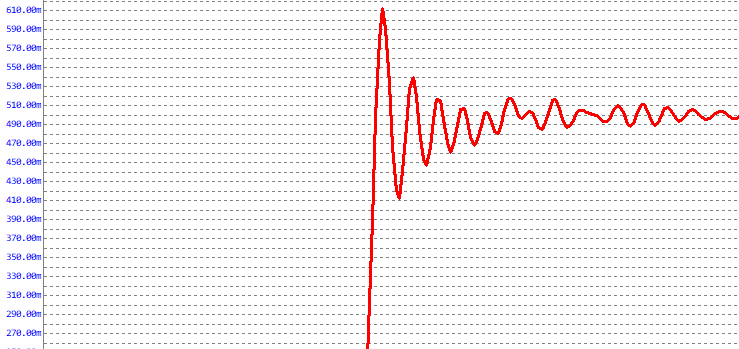
\includegraphics[width=0.45\textwidth]{EstimatingQ.png}
\caption{Transient Waveform for Estimating Q
}\label{fig:EstimatingQ}
\end{figure}


To estimate our circuit Q, we employ a technique called ring-down method
\cite{giangrandi}. Driving the circuit with a square wave much slower than the
expected resonance frequency of the LC network, we simply count the amount of
cycles it takes for the signal envelope to decay to rougly 50\% of the maximum
amplitude. Observing figure /ref{fig:EstimatingQ}, we see that the ringing dies
down in about 1 cycle. To get our Q estimate, we simply multiply this value by
approximate 4.53. This yields an approximate Q of 4.53 for our transmission
line. This seems a little lower than expected however, we can see that the
ringing is not as clean as we expected.
It is unsurprising that our non-linear circuit results in a fluctuating
impedance on the line causing reflections and is prone to generating harmonic
content.

By feeding in a 1Vpp Sine wave and measuring the frequency response of our
circuit, we see that many harmonics should be present in our line. Since we are
using this simulation to stand in place of a physical measurement, this
interferenece makes sense.

To repeat this process for our physical circuit is a good next step to confirm
the observed value of $Q \approx 5$.

\section{Next Steps}\label{sec:NextSteps}



\subsection{Verilog-A Module}

While we were able to draft a preliminary Verilog-A module for this project,
we were unable to fully debug, implement, or optimize this code.
Introductory literature exists explaining how these models are constructed
and used \cite{VerilogAFun}. There also exists literature specifically gear
toward creating RF models using Verilog-A\cite{VerilogARF}.
    
    




\subsection{Using varying physical circuit geometry}

figure \ref{fig:WeirdGeo} shows a possible implementation of pulse sharpening by
taking advantage of the circuit's physical geometry to produce further
non-linearities and mismatches in the circuit. This type of geometry should be
used with much higher frequencies than the designs we created for this report as
it relies on the the lines themselves to act as inductive components. This 
exploration may have several advantages including easier reproduction and less
resistive losses on the line due to lack of discrete inductors.

As an intermediate step, it may be beneficial to conduct further simulation with
varied inductance and parasitics to emulate the behavior of this topology.
"non-uniform" topologies have other applications and some examples can be found
in spectroscopy\cite{palmer2014performance} with use as antenna
tuners\cite{cure2012non} or even in bandpass filter
designs\cite{NonUniformBandpass}.


\begin{figure}[htb]
\centering
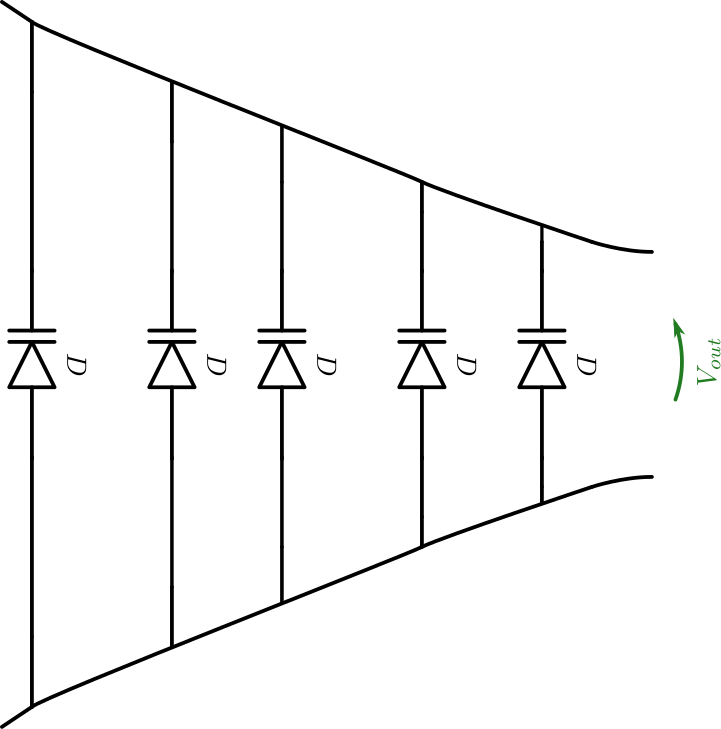
\includegraphics[width=0.45\linewidth]{WeirdNTLTGeometry.png}
\caption{\ Potential circuit geometry to be simulated and built going forward
}\label{fig:WeirdGeo}
\end{figure}


\section{ Conclusion} 









 
 
 
 
 
 
 
 
 
 
 
 
 

\bibliographystyle{IEEEtran}
\bibliography{mybib}

% Put all relevant IEEE articles we read here
% you can choose not to have a title for an appendix
% if you want by leaving the argument blank
%\begin{itemize}
%\item 
%\item 
%\item  
%\item 
%\end{itemize}
% use section* for acknowledgment



% Can use something like this to put references on a page
% by themselves when using endfloat and the captionsoff option.


% trigger a \newpage just before the given reference
% number - used to balance the columns on the last page
% adjust value as needed - may need to be readjusted if
% the document is modified later
%\IEEEtriggeratref{8}
% The "triggered" command can be changed if desired:
%\IEEEtriggercmd{\enlargethispage{-5in}}

% references section

% can use a bibliography generated by BibTeX as a .bbl file
% BibTeX documentation can be easily obtained at:
% http://www.ctan.org/tex-archive/biblio/bibtex/contrib/doc/
% The IEEEtran BibTeX style support page is at:
% http://www.michaelshell.org/tex/ieeetran/bibtex/
%
% <OR> manually copy in the resultant .bbl file
% set second argument of \begin to the number of references
% (used to reserve space for the reference number labels box)

% biography section
% 
% If you have an EPS/PDF photo (graphicx package needed) extra braces are
% needed around the contents of the optional argument to biography to prevent
% the LaTeX parser from getting confused when it sees the complicated
% \includegraphics command within an optional argument. (You could create
% your own custom macro containing the \includegraphics command to make things
% simpler here.)
%\begin{IEEEbiography}[{\includegraphics[width=1in,height=1.25in,clip,keepaspectratio]{mshell}}]{Michael Shell}
% or if you just want to reserve a space for a photo:



% if you will not have a photo at all:


% insert where needed to balance the two columns on the last page with
% biographies
%\newpage



% You can push biographies down or up by placing
% a \vfill before or after them. The appropriate
% use of \vfill depends on what kind of text is
% on the last page and whether or not the columns
% are being equalized.

%\vfill

% Can be used to pull up biographies so that the bottom of the last one
% is flush with the other column.
%\enlargethispage{-5in}



% that's all folks
\end{document}